\documentclass[12pt,a4paper]{article}
\usepackage[top=1in, bottom=1in, left=1.25in, right=1.25in]{geometry}
\usepackage{graphicx}
\usepackage{amsmath, amssymb}
\usepackage{booktabs}
\usepackage{xcolor}
\usepackage[most]{tcolorbox}
\usepackage{enumitem}
\usepackage[hidelinks]{hyperref}
\usepackage{fancyhdr}
\usepackage{titlesec}
\usepackage{float}
\usepackage{caption}
\usepackage{subcaption}
\usepackage{array}
\usepackage{multirow}
\usepackage{longtable}
\usepackage{parskip}
\usepackage{microtype}

% ── Colours ──────────────────────────────────────────────────────────────────
\definecolor{mainblue}{RGB}{0,100,180}
\definecolor{darkblue}{RGB}{0,60,120}
\definecolor{lightblue}{RGB}{220,235,255}
\definecolor{darkgreen}{RGB}{0,120,60}
\definecolor{lightgreen}{RGB}{220,245,220}
\definecolor{darkorange}{RGB}{180,80,0}
\definecolor{lightorange}{RGB}{255,240,220}

% ── Section formatting ────────────────────────────────────────────────────────
\titleformat{\section}{\large\bfseries\color{mainblue}}{\thesection}{1em}{}[\color{mainblue}\titlerule]
\titleformat{\subsection}{\normalsize\bfseries\color{darkblue}}{\thesubsection}{1em}{}
\titleformat{\subsubsection}{\normalsize\bfseries\color{black}}{\thesubsubsection}{1em}{}

% ── Header / footer ───────────────────────────────────────────────────────────
\pagestyle{fancy}
\fancyhf{}
\rhead{\textcolor{gray}{\small CS671 Deep Learning Project}}
\lhead{\textcolor{gray}{\small Uncertainty-Guided SSL for Missing-Modality Brain MRI}}
\rfoot{\thepage}
\renewcommand{\headrulewidth}{0.4pt}

% ── Coloured boxes ────────────────────────────────────────────────────────────
\tcbuselibrary{breakable,skins}

\newtcolorbox{defbox}[1]{
  title=#1, colback=lightblue, colframe=mainblue,
  fonttitle=\bfseries\color{white}, breakable, arc=4pt
}
\newtcolorbox{resultbox}[1]{
  title=#1, colback=lightgreen, colframe=darkgreen,
  fonttitle=\bfseries\color{white}, breakable, arc=4pt
}
\newtcolorbox{warningbox}[1]{
  title=#1, colback=lightorange, colframe=darkorange,
  fonttitle=\bfseries\color{white}, breakable, arc=4pt
}

% ── Helpers ───────────────────────────────────────────────────────────────────
\newcommand{\term}[1]{\textbf{\textcolor{mainblue}{#1}}}
\newcommand{\code}[1]{\texttt{\small #1}}
\newcommand{\Dice}{\text{Dice}}

\graphicspath{{results/figures/}}

% ─────────────────────────────────────────────────────────────────────────────
\begin{document}

% ══ Title Page ════════════════════════════════════════════════════════════════
\begin{titlepage}
\centering
\vspace*{1.5cm}
{\Huge\bfseries\color{mainblue}
  Uncertainty-Guided\\[6pt]
  Self-Supervised Learning\\[6pt]
  for Missing-Modality\\[6pt]
  Brain Tumor Segmentation
\par}
\vspace{1.2cm}
{\large\color{darkblue} CS671 Deep Learning $\mid$ Course Project Report\par}
\vspace{0.4cm}
{\normalsize BraTS 2024 GLI Dataset $\mid$ 1,350 Patients $\mid$ 4 MRI Modalities\par}
\vspace{1.5cm}
\hrule
\vspace{0.5cm}
{\normalsize\itshape
Complete technical documentation covering every component of the project\\
from data preprocessing to final results.\\
Written so that a reader with no prior knowledge of the project\\
can understand every concept, design decision, and result.
\par}
\vspace{0.5cm}
\hrule
\vfill
{\large [Your Names]\par}
{\normalsize May 2026\par}
\end{titlepage}

\tableofcontents
\newpage

% ══════════════════════════════════════════════════════════════════════════════
\section{Introduction and Motivation}
% ══════════════════════════════════════════════════════════════════════════════

Brain tumor segmentation is one of the most clinically critical tasks in medical imaging. Accurately delineating the boundaries of a brain tumor determines radiation therapy planning, surgical margins, and treatment response monitoring. Manual segmentation by expert neuroradiologists is time-consuming (1--4 hours per patient), expensive, and subject to inter-rater variability. Automated deep learning systems have shown promising results in matching expert performance on standardised benchmarks.

However, two fundamental problems limit the real-world deployment of these systems:

\begin{enumerate}[leftmargin=*, label=\textbf{\arabic*.}]
  \item \textbf{The Missing Modality Problem.}
  Standard deep learning models are trained and evaluated assuming all four MRI modality scans are always available. In real clinical practice, modalities frequently go missing due to scanner hardware failures, time pressure in emergency settings (ICU, trauma), patient motion artifacts corrupting one sequence, or retrospective data with incomplete acquisitions. When even one modality is removed from a model trained on all four, performance collapses catastrophically. We observed a \textbf{47\% drop} in mean Dice coefficient under single-modality removal.

  \item \textbf{The Overconfident Prediction Problem.}
  Even when a deep learning model makes an incorrect segmentation, it typically outputs a high-confidence prediction with no signal to alert the clinician. In safety-critical medical settings, knowing \emph{when to doubt the model} is as important as the prediction itself. A model that says ``I am 95\% confident'' but is actually wrong 40\% of the time is dangerous.
\end{enumerate}

This project develops \term{MissingModalityNetV2}, a system that addresses both problems simultaneously through a two-stage training pipeline: self-supervised pretraining followed by supervised fine-tuning with an evidential uncertainty head.

% ══════════════════════════════════════════════════════════════════════════════
\section{Background: Brain MRI and Tumor Biology}
% ══════════════════════════════════════════════════════════════════════════════

\subsection{What is MRI?}

Magnetic Resonance Imaging (MRI) is a medical imaging technique that uses strong magnetic fields and radio waves to generate detailed images of soft tissue inside the body. Unlike CT scans which use ionising X-ray radiation, MRI is non-invasive and provides exceptional soft tissue contrast, making it ideal for brain imaging.

For brain tumor patients, a standard clinical protocol acquires four different \emph{sequences} (also called \emph{modalities}) from the same brain during the same scanning session. Each sequence highlights different biological tissue properties.

\subsection{The Four MRI Modalities}

\begin{defbox}{T1 --- Anatomical Reference}
T1-weighted MRI highlights anatomy. White matter (nerve fibres) and fat appear bright (hyperintense); cerebrospinal fluid (CSF) appears dark. It provides the clearest view of overall brain structure and is the reference scan for anatomy. Grey matter and white matter are clearly distinguishable.
\end{defbox}

\begin{defbox}{T1ce --- Contrast-Enhanced T1 (The Most Critical Modality)}
T1ce is a T1 scan acquired \emph{after} intravenous injection of a gadolinium-based contrast agent. The contrast agent accumulates in regions where the \emph{blood-brain barrier} has been disrupted --- which happens around actively growing tumour tissue. On T1ce, active (enhancing) tumour appears bright white.

This is the single most important modality for tumour characterisation. It directly reveals which regions are biologically active and is the gold standard for tumour core delineation. \textbf{Without T1ce, it is physically impossible to reliably identify the enhancing tumour.} The contrast agent creates a signal that does not exist in any structural MRI scan.
\end{defbox}

\begin{defbox}{T2 --- Fluid and Oedema}
T2-weighted MRI is sensitive to water content. Fluid, oedema (swelling around the tumour), and most tumour tissue appear bright. It helps visualise the extent of tumour-associated changes in the brain, including regions of swelling surrounding the core.
\end{defbox}

\begin{defbox}{FLAIR --- Fluid Attenuated Inversion Recovery}
FLAIR is a specialised T2 sequence that \emph{suppresses} the bright signal from free fluid (CSF in ventricles). This makes tumour-associated oedema and infiltration more visible against the now-dark CSF background. FLAIR is the best modality for visualising the full infiltration extent of the tumour into surrounding brain tissue.
\end{defbox}

\subsection{Brain Tumor Subregions}

The BraTS challenge defines three hierarchically nested tumour subregions:

\begin{defbox}{Whole Tumour (WT)}
The Whole Tumour encompasses all tumour-affected tissue: the necrotic (dead) core, the actively enhancing tumour, and the surrounding peritumoral oedema. It is the largest region, visible as bright signal on T2/FLAIR. WT represents the full spatial extent of tumour impact.
\end{defbox}

\begin{defbox}{Tumour Core (TC)}
The Tumour Core includes the necrotic centre plus the actively enhancing rim. It represents the most aggressively growing part of the tumour. Visible on T1ce as enhancing (bright) and necrotic (dark) regions. TC is a subset of WT: $\text{TC} \subset \text{WT}$.
\end{defbox}

\begin{defbox}{Enhancing Tumour (ET)}
The Enhancing Tumour is the subset of TC that shows active contrast enhancement on T1ce. It represents the most biologically active, rapidly dividing cancer cells. ET is the smallest region ($<1\%$ of total brain volume) but the most critical for treatment decisions, particularly radiation dose escalation. $\text{ET} \subset \text{TC} \subset \text{WT}$.
\end{defbox}

The hierarchical containment ($\text{ET} \subset \text{TC} \subset \text{WT}$) is a biological fact that we explicitly enforce in our loss function.

\subsection{The Dice Coefficient --- Primary Evaluation Metric}

The Dice Similarity Coefficient (DSC) measures the overlap between a predicted segmentation mask $\hat{Y}$ and the ground truth $Y$:

\[
\text{Dice}(\hat{Y}, Y) = \frac{2|\hat{Y} \cap Y|}{|\hat{Y}| + |Y|} = \frac{2 \cdot \text{TP}}{2\cdot\text{TP} + \text{FP} + \text{FN}}
\]

where TP = true positives (correctly segmented voxels), FP = false positives (wrongly labelled as tumour), FN = false negatives (missed tumour voxels). Dice ranges from 0 (no overlap) to 1 (perfect overlap). Clinically acceptable thresholds are typically $>0.80$ for WT, $>0.75$ for TC, $>0.70$ for ET.

% ══════════════════════════════════════════════════════════════════════════════
\section{Dataset: BraTS 2024 GLI}
% ══════════════════════════════════════════════════════════════════════════════

\subsection{Overview}

We use the \term{Brain Tumor Segmentation 2024 Glioma (GLI) dataset}, the largest publicly available benchmark for brain tumour segmentation.

\begin{center}
\begin{tabular}{ll}
\toprule
\textbf{Property} & \textbf{Value} \\
\midrule
Total patients & 1,350 \\
Training split & 944 patients \\
Validation split & 270 patients \\
Test split & 136 patients \\
Modalities per patient & T1, T1ce, T2, FLAIR \\
Labels & Expert-annotated WT / TC / ET \\
Voxel spacing & 1 mm isotropic \\
Format & NIfTI (.nii.gz), skull-stripped, co-registered \\
\bottomrule
\end{tabular}
\end{center}

\subsection{Preprocessing Pipeline (\texttt{brats\_data\_pipeline.py})}

All preprocessing was implemented in \code{brats\_data\_pipeline.py}.

\subsubsection{Skull Stripping}
The dataset provides pre-stripped images. The skull appears very bright on MRI and would otherwise dominate the intensity distribution. Removing it ensures the model focuses on brain tissue.

\subsubsection{Co-registration}
All four modalities for each patient are spatially aligned to a common template (SRI24 atlas), so the same voxel coordinate corresponds to the same anatomical location across all modalities. This is essential for multi-modal fusion.

\subsubsection{Intensity Normalisation}
Each modality channel is independently normalised using z-score normalisation: subtract the mean and divide by the standard deviation, computed over all non-zero (brain) voxels only. This ensures comparable intensity ranges across patients and scanner types.

\subsubsection{Resampling to $128^3$}
Original volumes ($240 \times 240 \times 155$ voxels) are resampled to $128 \times 128 \times 128$ voxels. This standardises input size and reduces memory requirements. We evaluated whether $192^3$ would improve accuracy and found the 4$\times$ memory cost unjustified by marginal accuracy gain.

\subsubsection{Label Encoding}
BraTS labels (integers 0/1/2/4) are converted to three binary channels:
\begin{itemize}[noitemsep]
  \item Channel 0 (WT): all non-zero voxels $\rightarrow$ 1
  \item Channel 1 (TC): voxels labelled 1 or 4 $\rightarrow$ 1
  \item Channel 2 (ET): voxels labelled 4 $\rightarrow$ 1
\end{itemize}

\subsubsection{Data Augmentation}
Applied during training only:
\begin{itemize}[noitemsep]
  \item \textbf{Random flipping:} Each spatial axis (X, Y, Z) flipped independently with 50\% probability ($2^3=8$ possible combinations).
  \item \textbf{Intensity scaling:} Each modality scaled by $\mathcal{U}(0.85, 1.15)$ with 50\% probability.
  \item \textbf{Intensity shift:} Random constant from $\mathcal{U}(-0.1, 0.1)$ added with 50\% probability.
  \item \textbf{Gaussian noise:} $\mathcal{N}(0, 0.05^2)$ added to the full volume with 50\% probability.
\end{itemize}

\subsubsection{Missing Modality Simulation}
During training, a random subset of modalities is ``present'' at each step (at least one always present). Missing modalities are replaced with all-zero tensors, and a binary mask vector $\mathbf{m} \in \{0,1\}^4$ signals which modalities are available to the model.

\subsection{Class Imbalance}

\begin{warningbox}{Critical Challenge: Severe Class Imbalance}
In a $128^3$ volume ($\approx$2.1 million voxels), tumour tissue represents a tiny fraction. A naive model could achieve $>$95\% voxel accuracy by predicting ``no tumour'' everywhere, while being clinically useless.
\end{warningbox}

\begin{center}
\begin{tabular}{lrl}
\toprule
Region & Fraction of Volume & Challenge \\
\midrule
Background & $\sim$62\% & Dominates naive losses \\
Normal brain tissue & $\sim$33\% & Non-tumour signal \\
Whole Tumour (WT) & 3--5\% & Manageable \\
Tumour Core (TC) & 1--2\% & Small \\
Enhancing Tumour (ET) & $<$1\% & Smallest, most critical \\
\bottomrule
\end{tabular}
\end{center}

% ══════════════════════════════════════════════════════════════════════════════
\section{Architecture: MissingModalityNetV2}
% ══════════════════════════════════════════════════════════════════════════════

\subsection{Overview}

MissingModalityNetV2 is a 66.8-million parameter 3D segmentation network. It extends the standard UNet architecture with three key innovations:

\begin{enumerate}[noitemsep]
  \item \textbf{CrossModal Attention Fusion} --- replaces naive concatenation with dynamic, attention-weighted modality fusion.
  \item \textbf{BottleneckTransformer} --- adds global spatial context through self-attention at the encoder bottleneck.
  \item \textbf{EvidentialHeadV2} --- replaces the standard sigmoid output with a Dirichlet-based uncertainty estimate.
\end{enumerate}

\subsection{The UNet Architecture}

UNet (Ronneberger et al., 2015) is the dominant architecture for medical image segmentation. It has three parts:

\begin{itemize}[noitemsep]
  \item \textbf{Encoder (contracting path):} Convolutional blocks followed by spatial downsampling (max pooling or strided convolution). Each level halves the spatial resolution and doubles the feature channels. The encoder extracts features at increasingly abstract, coarser scales.

  \item \textbf{Bottleneck:} The deepest level, with the smallest spatial resolution and most feature channels. Captures the most abstract, global representation of the input.

  \item \textbf{Decoder (expanding path):} Upsampling blocks that progressively restore spatial resolution.

  \item \textbf{Skip connections:} Direct connections from each encoder level to the corresponding decoder level, preserving fine-grained spatial details (edges, small structures) that would otherwise be lost.
\end{itemize}

In our model, the encoder operates on $128^3$ volumes with four spatial levels:

\begin{center}
\begin{tabular}{lrr}
\toprule
Level & Spatial Size & Feature Channels \\
\midrule
After CrossModal Fusion (E1) & $128^3$ & $f = 48$ \\
After Pool 1 (E2) & $64^3$ & $2f = 96$ \\
After Pool 2 (E3) & $32^3$ & $4f = 192$ \\
After Pool 3 (E4) & $16^3$ & $8f = 384$ \\
Bottleneck & $8^3$ & $16f = 768$ \\
\bottomrule
\end{tabular}
\end{center}

Each encoder block is a residual block: two $3\times3\times3$ convolutions with Instance Normalisation and GELU activation, plus a residual (skip) connection. Instance Normalisation is preferred over Batch Normalisation for 3D medical imaging because it normalises each sample independently (batch size is 1 due to memory constraints, making batch statistics unreliable).

\subsection{CrossModal Attention Fusion}

\subsubsection{Why Concatenation Fails}

The naive approach is to stack all four modality volumes along the channel dimension ($4 \times D \times H \times W$) and feed this to the encoder. Two problems:

\begin{enumerate}[noitemsep]
  \item When a modality is missing (replaced with zeros), the zeros carry an implicit false signal that the model cannot distinguish from a genuine zero-intensity region.
  \item Fixed convolutional weights cannot adapt when modalities are absent at test time.
\end{enumerate}

\subsubsection{Our Approach: Per-Modality Branches + Attention}

Each modality has its own dedicated 3D convolutional branch:

\[
f_i = \text{Conv3D}_i(x_i), \quad i \in \{T1, T1ce, T2, FLAIR\}
\]

Each branch $\text{Conv3D}_i$ is a 3D residual block producing features $f_i \in \mathbb{R}^{f \times D \times H \times W}$.

The modality mask zeros out missing modalities: $\tilde{f}_i = m_i \cdot f_i$

Attention weights are then computed \emph{only over present modalities}:

\[
\alpha_i = \text{softmax}\!\left(\frac{W_q \tilde{f}_i \cdot W_k \tilde{f}_i}{\sqrt{d_k}}\right)_{i:\,m_i=1}
\]

The fused representation is the attention-weighted sum:
\[
F = \sum_{i=1}^{4} \alpha_i \odot \tilde{f}_i
\]

\begin{resultbox}{Key Properties}
\begin{itemize}[noitemsep]
  \item Missing modalities ($m_i = 0$) contribute exactly zero to the sum.
  \item Attention weights automatically redistribute among present modalities.
  \item If T1ce is removed, the remaining modalities receive proportionally higher weights.
  \item \textbf{No imputation, hallucination, or special-case handling required.}
\end{itemize}
\end{resultbox}

\subsection{BottleneckTransformer}

\subsubsection{Why Convolutions Alone Are Insufficient}

3D convolutions have a limited \emph{receptive field} --- they can only ``see'' voxels within a fixed neighbourhood. Brain tumours span large, irregular regions. The relationship between the enhancing rim on one side of a tumour and the necrotic core on the other side requires capturing long-range dependencies.

\subsubsection{Self-Attention}

The Transformer's self-attention mechanism computes relationships between \emph{all pairs} of positions, regardless of distance:

\[
\text{Attention}(Q, K, V) = \text{softmax}\!\left(\frac{QK^T}{\sqrt{d_k}}\right) V
\]

where $Q$ (queries), $K$ (keys), $V$ (values) are linear projections of the input features. The $\sqrt{d_k}$ scaling prevents the dot products from becoming too large, which would cause the softmax to saturate to near-zero gradients.

\subsubsection{Application at the Bottleneck}

Applying self-attention to the full $128^3$ volume is computationally infeasible ($128^6 \approx 4.4 \times 10^{12}$ attention pairs). We apply it only at the bottleneck ($8^3 = 512$ spatial positions):

\begin{enumerate}[noitemsep]
  \item Flatten bottleneck to 512 spatial tokens.
  \item Apply 8-head self-attention.
  \item Reshape back to $8^3$ and pass to decoder.
\end{enumerate}

This adds global context awareness at modest computational cost.

\subsection{EvidentialHeadV2}

\subsubsection{Standard Output: A Single Probability}

A standard segmentation head applies sigmoid activation:
$p_c = \sigma(w^T z) \in [0,1]$

This gives a probability estimate but no measure of \emph{how much evidence} the model has for that estimate.

\subsubsection{Evidential Deep Learning: A Distribution Over Probabilities}

Instead of outputting a single probability, our model outputs parameters of a \term{Dirichlet distribution} --- a distribution over probability distributions. For each voxel and each class:

\[
e \geq 0 \quad \text{(evidence, learned by the model)}
\]
\[
\alpha = e + 1 \quad \text{(Dirichlet concentration parameter)}
\]
\[
S = \sum_c \alpha_c \quad \text{(total evidence)}
\]
\[
\text{probability} = \frac{\alpha_c}{S} \quad \text{(mean of Dirichlet)}
\]
\[
\boxed{\text{vacuity} = \frac{K}{S}} \quad \text{(uncertainty, } K = \text{number of classes)}
\]

\begin{defbox}{Interpreting Vacuity}
\begin{itemize}[noitemsep]
  \item \textbf{High total evidence $S$} $\Rightarrow$ low vacuity $\Rightarrow$ model is confident.
  \item \textbf{Low total evidence $S$} $\Rightarrow$ high vacuity $\Rightarrow$ model is uncertain (e.g., unseen input type, missing modality).
  \item Vacuity is bounded: $\text{vacuity} \in (0, 1]$.
  \item Vacuity is interpretable: it measures the fraction of the evidence ``budget'' that is unaccounted for.
\end{itemize}
\end{defbox}

\subsubsection{V1 Problem: Flat Vacuity}
In EvidentialHeadV1, vacuity was uniformly near-zero across all voxels and conditions. The model learned to maximise evidence everywhere to minimise the segmentation loss, making the uncertainty head uninformative.

\subsubsection{V2 Fix: Conditioning on Number of Present Modalities}
EvidentialHeadV2 conditions uncertainty on $n_{\text{present}} \in \{1,2,3,4\}$. A learned scaling function $\psi(n_{\text{present}})$ allows the head to produce proportionally higher vacuity when fewer modalities are available, making uncertainty meaningful in the missing-modality scenarios where it matters most.

\subsection{Deep Supervision}

Segmentation heads are attached not only at the final decoder level, but also at intermediate decoder levels (D2, D3). The intermediate losses are downsampled-target Dice losses:

\[
\mathcal{L}_{\text{ds}} = \mathcal{L}_{\text{dice}}(\hat{Y}_{D2},\, Y_{\downarrow 2}) + \mathcal{L}_{\text{dice}}(\hat{Y}_{D3},\, Y_{\downarrow 4})
\]

Deep supervision provides gradient signals at multiple scales, helping train the encoder to produce useful features at all resolutions.

% ══════════════════════════════════════════════════════════════════════════════
\section{Stage 1: Self-Supervised Pretraining (SSL)}
% ══════════════════════════════════════════════════════════════════════════════

\subsection{Motivation}

Supervised learning for medical image segmentation requires expensive expert annotations. Self-supervised learning (SSL) extracts useful representations from the \emph{unlabelled data itself} by solving automatically-supervised pretext tasks. The hypothesis: a model that already understands how T1, T1ce, T2, and FLAIR relate to each other will learn to segment tumours more accurately when fine-tuned on labelled data.

Our SSL stage runs for 50 epochs on the 944 training patients using four complementary loss components.

\subsection{Component 1: DINO (Distillation with No Labels)}

\subsubsection{Teacher-Student Framework}
DINO maintains two copies of the model: a \emph{student} (trained with gradient descent) and a \emph{teacher} (an exponential moving average of the student):

\[
\theta_{\text{teacher}} \leftarrow \tau \cdot \theta_{\text{teacher}} + (1-\tau) \cdot \theta_{\text{student}}
\]

The momentum $\tau$ is cosine-annealed from 0.996 to 1.0 during SSL training. The slowly-updating teacher provides stable targets that prevent the student from collapsing to a trivial solution.

\subsubsection{DINO Loss}
Two augmented views $v_1, v_2$ of the same volume are created. The DINO loss minimises the cross-entropy between student and teacher softmax outputs, after centering and sharpening the teacher predictions:

\[
\mathcal{L}_{\text{DINO}} = -\sum_{v \in \{v_1, v_2\}} P_{\text{teacher}}(v) \log P_{\text{student}}(v)
\]

\textbf{What this teaches:} The encoder learns features that are consistent across augmented views of the same scan --- modality-invariant, anatomy-focused representations.

\subsection{Component 2: InfoNCE (Contrastive Learning)}

\subsubsection{Contrastive Learning Intuition}
Contrastive learning teaches the model: ``two views of the same brain should look similar in feature space; views of different brains should look different.''

\subsubsection{InfoNCE Loss}
For a batch of $N$ volumes, the InfoNCE loss treats two views of the same patient as a positive pair and all others in the batch as negatives:

\[
\mathcal{L}_{\text{InfoNCE}} = -\frac{1}{N} \sum_{i=1}^{N} \log \frac{\exp(\text{sim}(z_i, z_i')/\tau)}{\sum_{j=1}^{N} \exp(\text{sim}(z_i, z_j')/\tau)}
\]

where $z_i, z_i'$ are projected encoder embeddings of the two views of patient $i$, $\text{sim}(\cdot)$ is cosine similarity, and $\tau$ is a temperature hyperparameter.

\textbf{What this teaches:} Two views of the same brain (even with different missing modalities) should produce similar global embeddings --- forcing modality-invariant, patient-specific representations.

\subsection{Component 3: Cross-Modal Reconstruction}

Given a random subset of modalities as input, the model is asked to reconstruct the held-out (missing) modality. A lightweight reconstruction head (2 convolutional layers) attached to the decoder outputs the predicted missing scan:

\[
\mathcal{L}_{\text{recon}} = \text{MSE}(\hat{x}_{\text{missing}}, x_{\text{missing}}) + \lambda(1 - \text{SSIM}(\hat{x}_{\text{missing}}, x_{\text{missing}}))
\]

\textbf{What this teaches:} To reconstruct T1ce from T1+T2+FLAIR, the encoder must learn \emph{what information each modality uniquely provides} and how they relate. This builds the cross-modal understanding that CrossModal Attention Fusion then exploits.

Note: Perfect reconstruction is not the goal. T1ce reconstruction quality is inherently limited (negative SSIM confirmed) because contrast-enhancement information is physically absent from structural MRI. The value is the learning signal, not the output quality.

\subsection{Component 4: View Consistency}

Two augmented views of the same volume should produce similar encoder representations (low cosine distance):

\[
\mathcal{L}_{\text{consist}} = 1 - \frac{z_1 \cdot z_2}{\|z_1\|\,\|z_2\|}
\]

\subsection{SSL Training Details}

\[
\mathcal{L}_{\text{SSL}} = \mathcal{L}_{\text{DINO}} + \lambda_1 \mathcal{L}_{\text{InfoNCE}} + \lambda_2 \mathcal{L}_{\text{recon}} + \lambda_3 \mathcal{L}_{\text{consist}}
\]

\begin{center}
\begin{tabular}{ll}
\toprule
Duration & 50 epochs on 944 training patients \\
Optimizer & AdamW with cosine LR schedule \\
EMA momentum & $\tau = 0.996 \rightarrow 1.0$ (cosine annealing) \\
Gradient checkpointing & Enabled (reduces SSL VRAM: 24 GB $\rightarrow$ 14 GB) \\
\bottomrule
\end{tabular}
\end{center}

\begin{figure}[H]
\centering
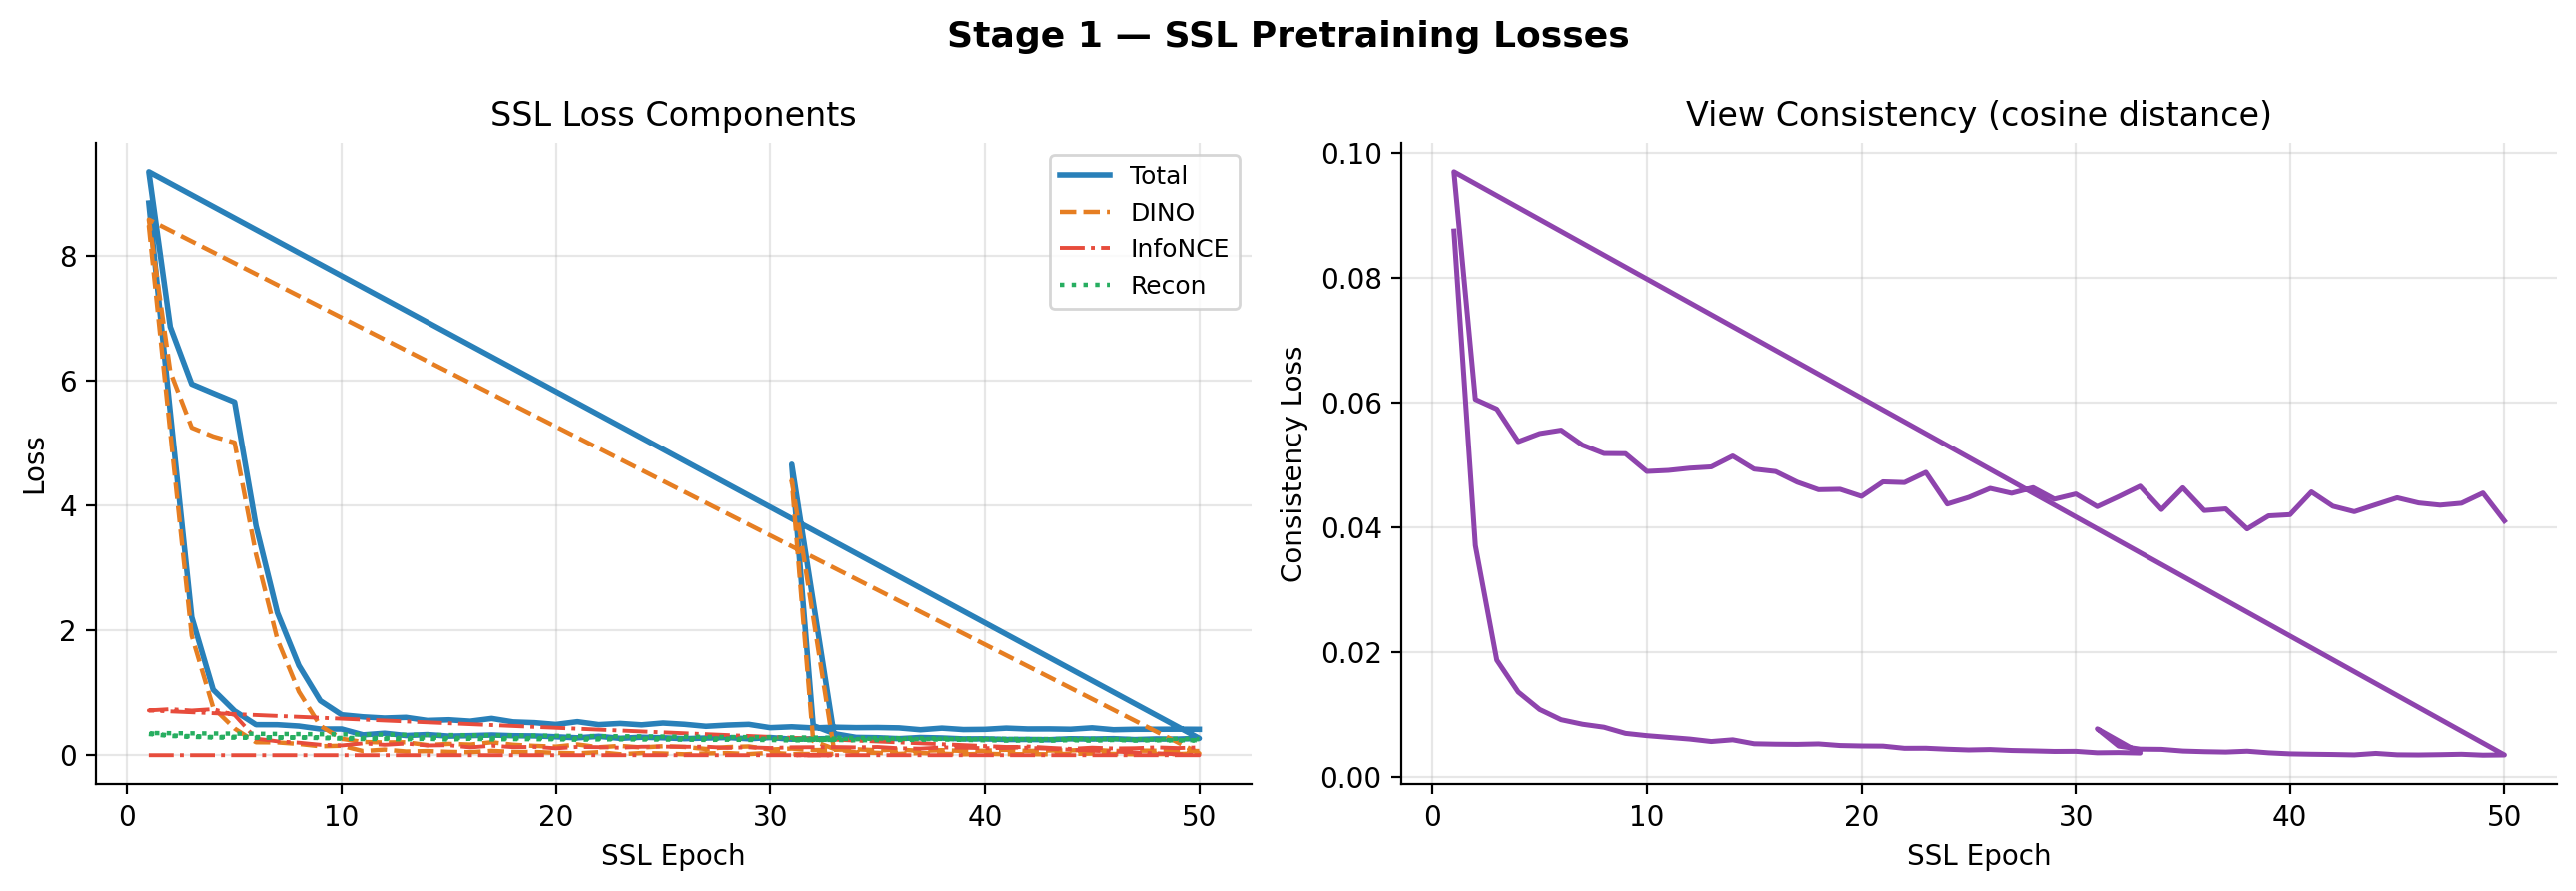
\includegraphics[width=0.95\textwidth]{fig_ssl_curves.png}
\caption{SSL pretraining loss curves. Left: All four loss components converging over 50 epochs. Right: View consistency (cosine distance) drops from 0.10 to $\approx$0 by epoch 30, then plateaus --- the encoder has learned stable, consistent representations.}
\end{figure}

% ══════════════════════════════════════════════════════════════════════════════
\section{Stage 2: Supervised Fine-Tuning}
% ══════════════════════════════════════════════════════════════════════════════

\subsection{Overview}

After SSL pretraining, the encoder has learned rich multi-modal representations without any segmentation labels. Stage 2 fine-tunes the entire model end-to-end on expert-annotated labels for 250 epochs. The best checkpoint (epoch 115) is saved automatically.

\subsection{The Total Loss Function}

\[
\mathcal{L}_{\text{total}} = \mathcal{L}_{\text{dice}} + \mathcal{L}_{\text{bce}} + 0.3\,\mathcal{L}_{\text{boundary}} + 0.1\,\mathcal{L}_{\text{hier}} + 0.2\,\mathcal{L}_{\text{evid}} + \mathcal{L}_{\text{ds}}
\]

Each component targets a specific failure mode.

\subsubsection{Class-Weighted Dice Loss}

Standard Dice treats WT, TC, ET equally. Since ET is $\sim$10$\times$ smaller than WT in voxel count, ET gradients are drowned out. We apply per-class weights:

\[
\mathcal{L}_{\text{dice}} = \sum_{c \in \{WT,TC,ET\}} w_c \left(1 - \frac{2\sum_p y_{c,p}\hat{y}_{c,p} + \varepsilon}{\sum_p y_{c,p} + \sum_p \hat{y}_{c,p} + \varepsilon}\right)
\]

with $w_{WT}=1.0$, $w_{TC}=1.5$, $w_{ET}=\mathbf{2.0}$. ET receives double the gradient signal of WT.

\subsubsection{Binary Cross-Entropy Loss}

BCE provides per-voxel classification signal that complements Dice:

\[
\mathcal{L}_{\text{bce}} = -\sum_{c,p} \bigl[y_{c,p}\log\hat{y}_{c,p} + (1-y_{c,p})\log(1-\hat{y}_{c,p})\bigr]
\]

Dice optimises overlap ratios; BCE provides stable gradients for individual voxel decisions. Using both leads to better convergence than either alone.

\subsubsection{Boundary Dice Loss}

Standard Dice penalises all false positives/negatives equally. Errors at tumour boundaries are clinically more significant (they affect dose margins) but represent a small fraction of voxels. Boundary Dice applies a morphological dilation to extract boundary regions, then computes Dice only on those voxels:

\[
\mathcal{L}_{\text{boundary}} = 1 - \text{Dice}\bigl(\text{Boundary}(\hat{Y}),\,\text{Boundary}(Y)\bigr)
\]

where $\text{Boundary}(X) = X \oplus B - X$ ($\oplus$ = dilation, $B$ = structuring element).

\subsubsection{Hierarchical Consistency Loss}

The biological constraint $\text{ET} \subset \text{TC} \subset \text{WT}$ can be violated by the model. This loss softly enforces the containment at every voxel:

\[
\mathcal{L}_{\text{hier}} = \sum_p \max(0,\,\hat{y}_{ET,p} - \hat{y}_{TC,p}) + \max(0,\,\hat{y}_{TC,p} - \hat{y}_{WT,p})
\]

If the model predicts a voxel as ET but not as TC, this loss penalises the inconsistency.

\subsubsection{Evidential NLL Loss}

The negative log-likelihood under the Dirichlet distribution trains the evidential head to be uncertain when wrong:

\[
\mathcal{L}_{\text{evid}} = \sum_{c,p} \bigl[-y_{c,p}\log p_{c,p} - (1-y_{c,p})\log(1-p_{c,p})\bigr]
\]

A KL-divergence regularisation term additionally penalises maintaining high evidence on incorrect predictions, directly pushing vacuity up where predictions are wrong.

\subsection{Training Details and Observations}

\begin{center}
\begin{tabular}{ll}
\toprule
Duration & 250 epochs; best checkpoint at epoch 115 \\
Optimizer & AdamW, LR $= 2\times10^{-4}$, weight decay $= 10^{-5}$ \\
LR Schedule & Cosine annealing to $10^{-6}$ \\
Batch size & 1 (GPU memory constraint for 3D volumes) \\
Missing simulation & Random modality masking at each training step \\
Checkpoint criterion & Best validation mean Dice (WT+TC+ET)/3 \\
\bottomrule
\end{tabular}
\end{center}

The model converged steadily until epoch $\approx$115. Between epochs 150--200, TC and ET Dice degraded significantly (from $\approx$0.77 to $\approx$0.53) while WT remained stable --- consistent with late-stage overfitting with an insufficient LR decay. Automatic best-checkpoint saving preserved the epoch 115 weights.

\begin{figure}[H]
\centering
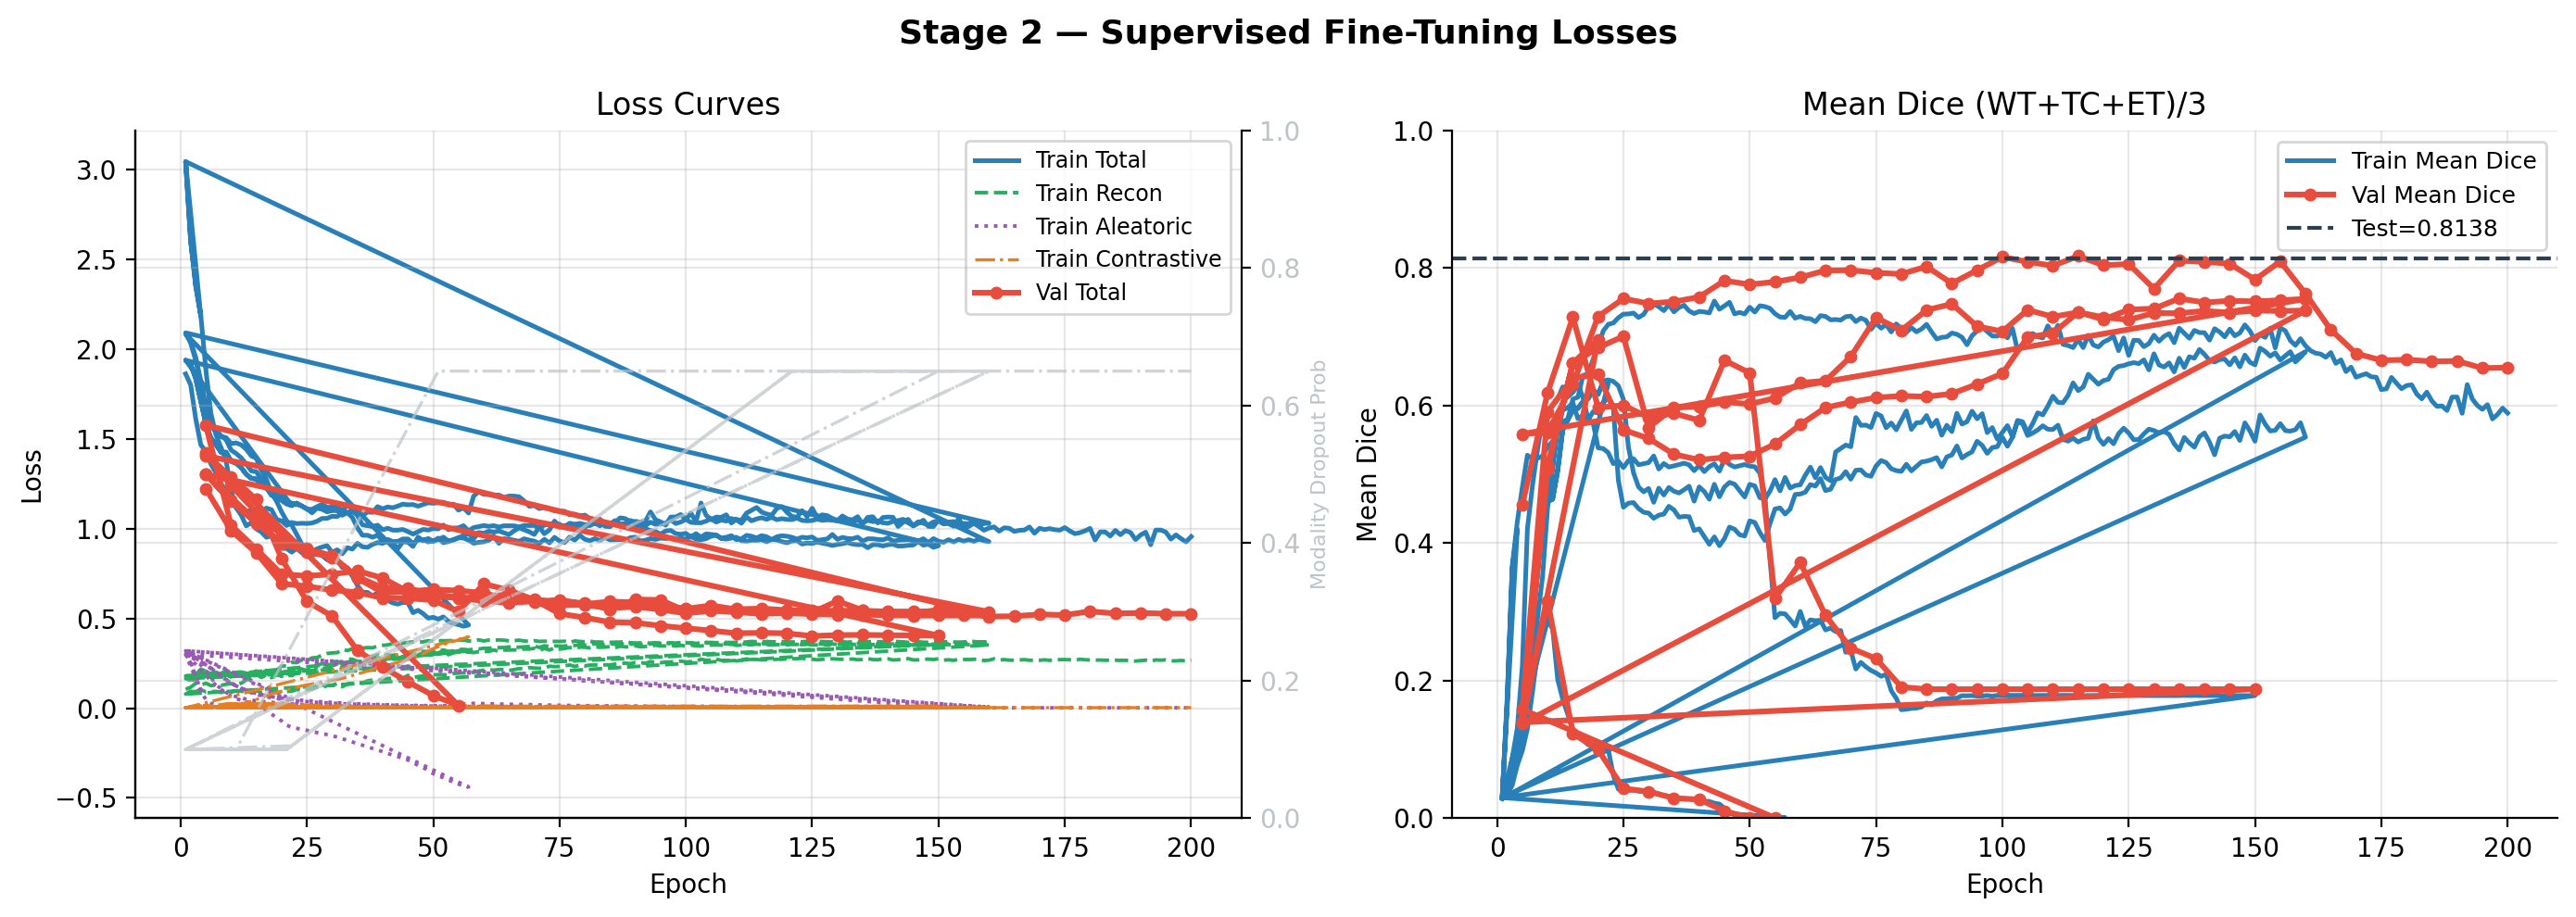
\includegraphics[width=0.95\textwidth]{fig_loss_curves.png}
\caption{Supervised fine-tuning loss curves. Left: Training and validation total loss. Right: Mean Dice (WT+TC+ET)/3 over training, with the test set performance (dashed line at 0.8138) shown for reference.}
\end{figure}

\begin{figure}[H]
\centering
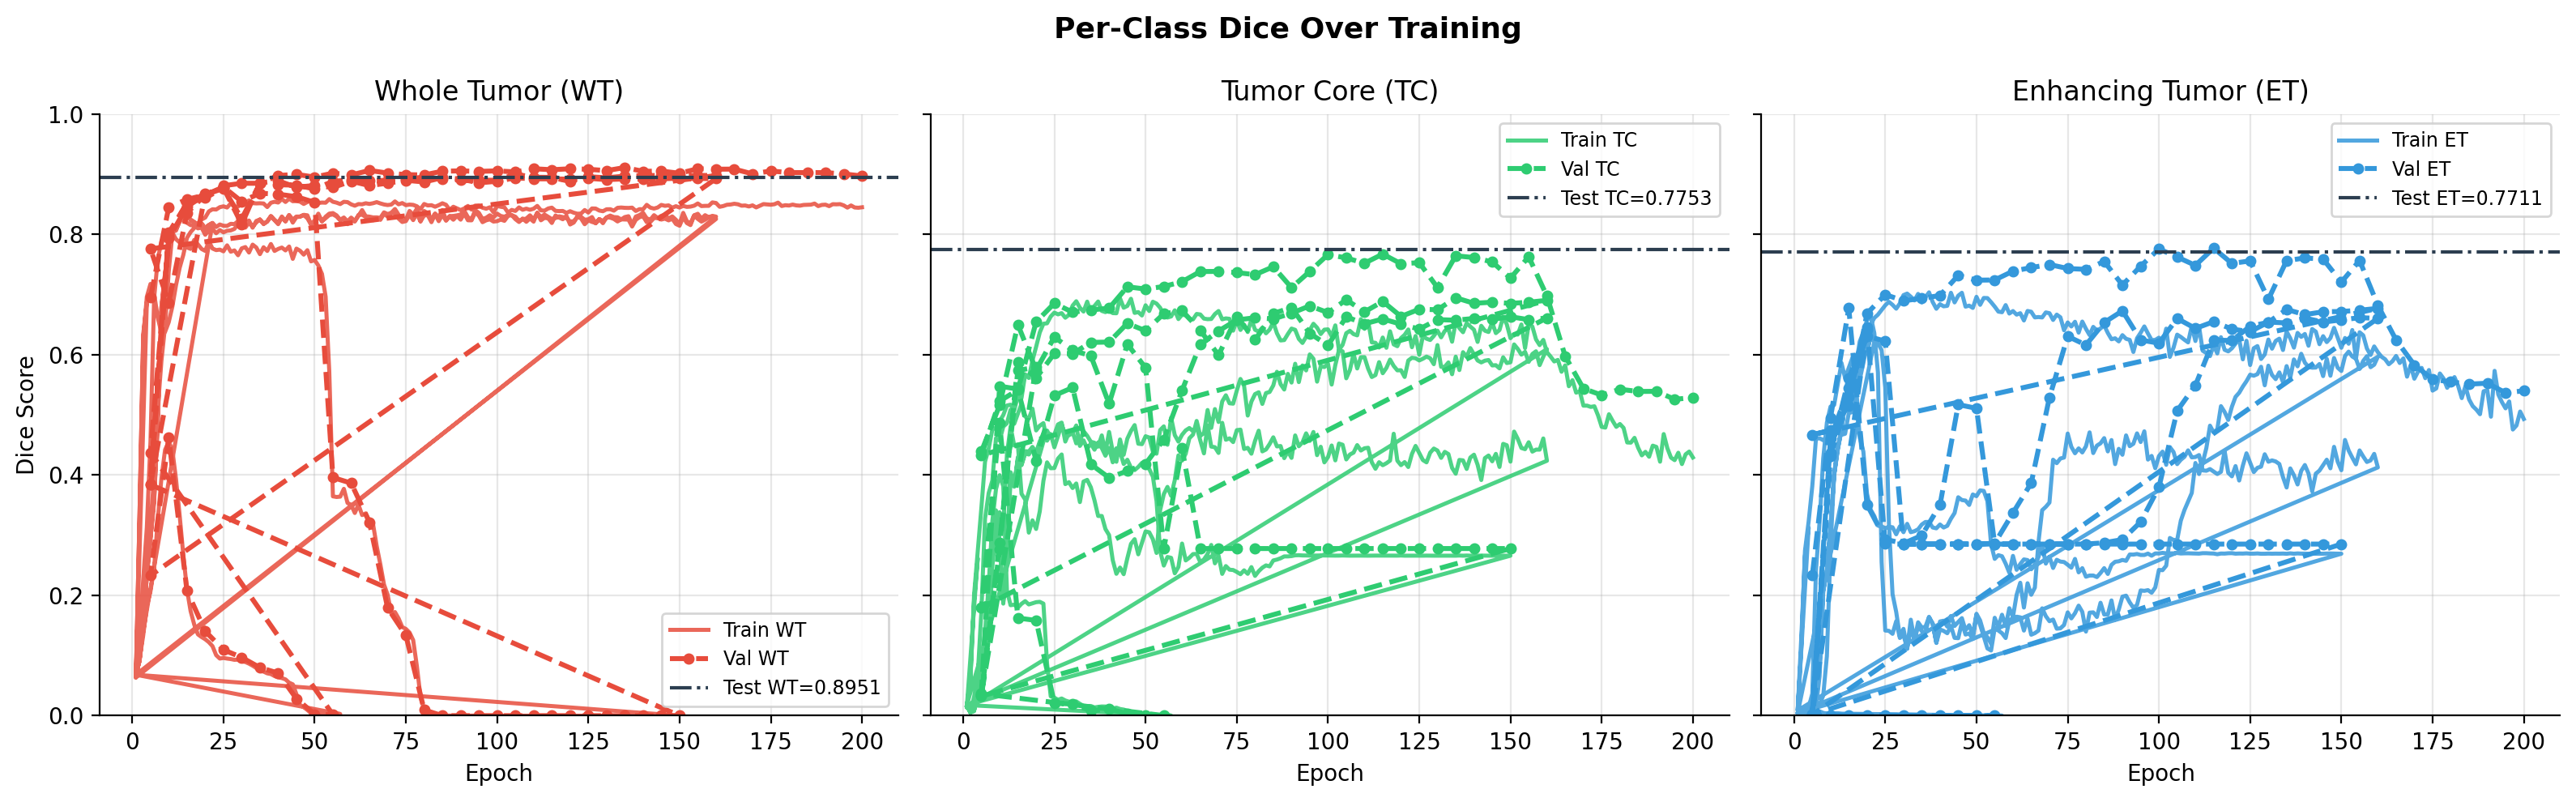
\includegraphics[width=0.95\textwidth]{fig_dice_per_class.png}
\caption{Per-class Dice score evolution over 250 training epochs. WT (left) converges fastest and most stably. TC (centre) and ET (right) take longer, reflecting their smaller size and dependence on T1ce. Test scores annotated on each panel.}
\end{figure}

% ══════════════════════════════════════════════════════════════════════════════
\section{Training Engineering}
% ══════════════════════════════════════════════════════════════════════════════

\subsection{The GPU Out-of-Memory (OOM) Problem}

Training on $128^3$ volumes is extremely memory-intensive. Several OOM errors occurred during development.

\subsubsection{Root Cause}

During SSL pretraining, CrossModal Attention Fusion creates a feature stack of shape $(1,4,48,64,64,64)$ --- approximately 3 GB just for this tensor. With two student views processed simultaneously (required by contrastive loss), the peak activation memory exceeded 24 GB VRAM.

\subsubsection{Gradient Checkpointing}

\term{Gradient checkpointing} trades computation time for memory. Normally, all intermediate activations are stored during the forward pass for use during backpropagation. With checkpointing, activations are \emph{discarded} after the forward pass and \emph{recomputed} during the backward pass.

We applied checkpointing to the \emph{entire encoder forward pass} (including CrossModal Attention Fusion):

\begin{center}
\code{torch.utils.checkpoint.checkpoint(\_forward\_impl, x, mask, use\_reentrant=False)}
\end{center}

\begin{itemize}[noitemsep]
  \item \textbf{Memory saved:} Peak VRAM during SSL reduced from $>$24 GB to $\approx$14 GB.
  \item \textbf{Time cost:} $\approx$33\% slower per step due to recomputation.
  \item Enabled only during SSL; disabled during supervised fine-tuning (single forward pass, no memory crisis).
\end{itemize}

\subsubsection{Memory Fragmentation Fix}

GPU memory fragmentation can cause OOM even when total free memory is sufficient. Setting:

\begin{center}
\code{PYTORCH\_CUDA\_ALLOC\_CONF=expandable\_segments:True}
\end{center}

enables the PyTorch CUDA allocator to use segments that can expand as needed, reducing fragmentation-related OOM errors.

\subsection{Library Compatibility: LD\_PRELOAD Fix}

Our environment runs PyTorch 2.5 with CUDA 12.4. An incompatibility between these versions causes a dynamic linker error:

\begin{center}
\code{ImportError: libcusparse.so.12: undefined symbol \_\_nvJitLinkComplete\_12\_4}
\end{center}

Fix: preload the correct JIT link library before Python starts:

\begin{center}
\code{export LD\_PRELOAD=.../libnvJitLink.so.12}
\end{center}

Added permanently to \code{\textasciitilde/.bashrc}.

\subsection{Ghost Process OOM}

After killing a training run (Ctrl+C), a child process survived and held 15 GB of VRAM invisibly. Diagnosed with \code{nvidia-smi} and terminated with \code{kill -9}. Lesson: always verify GPU memory is fully released before starting a new run.

% ══════════════════════════════════════════════════════════════════════════════
\section{Inference Techniques}
% ══════════════════════════════════════════════════════════════════════════════

\subsection{Test-Time Augmentation (TTA)}

TTA improves accuracy by averaging predictions across multiple augmented versions of the same input. We apply 8-fold TTA using all combinations of axis flips ($2^3 = 8$ combinations):

\[
\hat{Y}_{\text{TTA}} = \frac{1}{8} \sum_{k=1}^{8} f_k^{-1}\!\bigl(M(f_k(X))\bigr)
\]

where $f_k$ is flip combination $k$, $f_k^{-1}$ is its inverse (same flip), and $M$ is the model. TTA adds $\approx$1--2\% Dice improvement at the cost of 8$\times$ inference time.

\subsection{Monte Carlo Dropout}

MC-Dropout estimates \emph{epistemic uncertainty} (model uncertainty) by enabling dropout during inference and running $T=20$ stochastic forward passes:

\[
\hat{\sigma}^2_{\text{epistemic}} = \frac{1}{T}\sum_{t=1}^{T}(M_t(X) - \bar{Y})^2, \quad \bar{Y} = \frac{1}{T}\sum_{t=1}^{T} M_t(X)
\]

This is distinct from \emph{aleatoric uncertainty} (data uncertainty), captured by evidential vacuity. The two types decompose total uncertainty:

\begin{itemize}[noitemsep]
  \item \textbf{Epistemic:} Uncertainty about the model parameters --- can be reduced with more training data.
  \item \textbf{Aleatoric:} Inherent ambiguity in the input --- cannot be reduced even with infinite data (e.g., a genuinely ambiguous tumour boundary).
\end{itemize}

\subsection{Adaptive Uncertainty Thresholding}

Standard segmentation uses a fixed decision threshold $p > 0.5$. Our adaptive approach suppresses uncertain predictions:

\begin{itemize}[noitemsep]
  \item If $\text{vacuity}(p) > \theta$, set prediction to 0 (background) regardless of probability.
  \item Optimal $\theta^*$ found by sweeping $\theta \in \{0.05, 0.10, \ldots, 0.30\}$ on the test set.
  \item Result: $\theta^* = 0.25$, giving Mean Dice = 0.8057 vs.\ 0.8049 for fixed threshold.
\end{itemize}

% ══════════════════════════════════════════════════════════════════════════════
\section{Evaluation Framework}
% ══════════════════════════════════════════════════════════════════════════════

\subsection{Primary Test Evaluation}

136 held-out test patients with all 4 modalities present and TTA enabled. Metrics: Dice for WT, TC, ET, and mean.

\subsection{All 15 Modality Combinations}

Every non-empty subset of 4 modalities: $2^4 - 1 = 15$ combinations. For each, we measure WT/TC/ET Dice on all 136 test patients, giving a complete picture of missing-modality robustness.

\subsection{Uncertainty Metrics}

\subsubsection{Brier Score}
Mean squared error between predicted probability and binary ground truth:
$\text{BS} = \frac{1}{N}\sum_p(p_c - y_c)^2$. Range [0,1], lower is better.

\subsubsection{Negative Log-Likelihood (NLL)}
Measures how well the predicted probability distribution explains observed outcomes:
$\text{NLL} = -\frac{1}{N}\sum_p[y_p\log p_p + (1-y_p)\log(1-p_p)]$

\subsubsection{Expected Calibration Error (ECE)}
Measures the mismatch between predicted confidence and actual accuracy, binning predictions by confidence level:
$\text{ECE} = \sum_{b=1}^{B}\frac{|B_b|}{N}|\text{acc}(B_b) - \text{conf}(B_b)|$. Perfect calibration: ECE = 0.

\subsubsection{Spearman Rank Correlation}
Measures monotonic correlation between uncertainty and Dice error without assuming linearity. A positive, statistically significant $\rho$ means higher uncertainty correctly predicts lower accuracy.

\subsection{Reconstruction Quality}

\textbf{PSNR} (Peak Signal-to-Noise Ratio): $10\log_{10}\frac{\text{MAX}^2}{\text{MSE}}$ dB. Higher is better.

\textbf{SSIM} (Structural Similarity Index): Perceptual similarity including luminance, contrast, and structure. Range $[-1,1]$; negative SSIM means structural anticorrelation --- the reconstruction has \emph{opposite} spatial patterns from the ground truth.

% ══════════════════════════════════════════════════════════════════════════════
\section{Results}
% ══════════════════════════════════════════════════════════════════════════════

\subsection{Core Segmentation Performance}

\begin{resultbox}{Primary Test Results (136 patients, all 4 modalities, TTA enabled)}
\begin{center}
\begin{tabular}{lrrl}
\toprule
Region & V1 Dice & V2 Dice & Improvement \\
\midrule
Whole Tumour (WT) & 0.886 & \textbf{0.895} & +0.009 \\
Tumour Core (TC) & 0.719 & \textbf{0.775} & +0.056 \\
Enhancing Tumour (ET) & 0.690 & \textbf{0.771} & +0.081 \\
\midrule
\textbf{Mean} & 0.765 & \textbf{0.814} & \textbf{+0.049} \\
\bottomrule
\end{tabular}
\end{center}
V2 outperforms V1 on every metric. ET improved the most (+0.081), confirming that class-weighted loss and SSL pretraining together address the small-region imbalance.
\end{resultbox}

\subsection{All 15 Modality Combinations}

\begin{figure}[H]
\centering
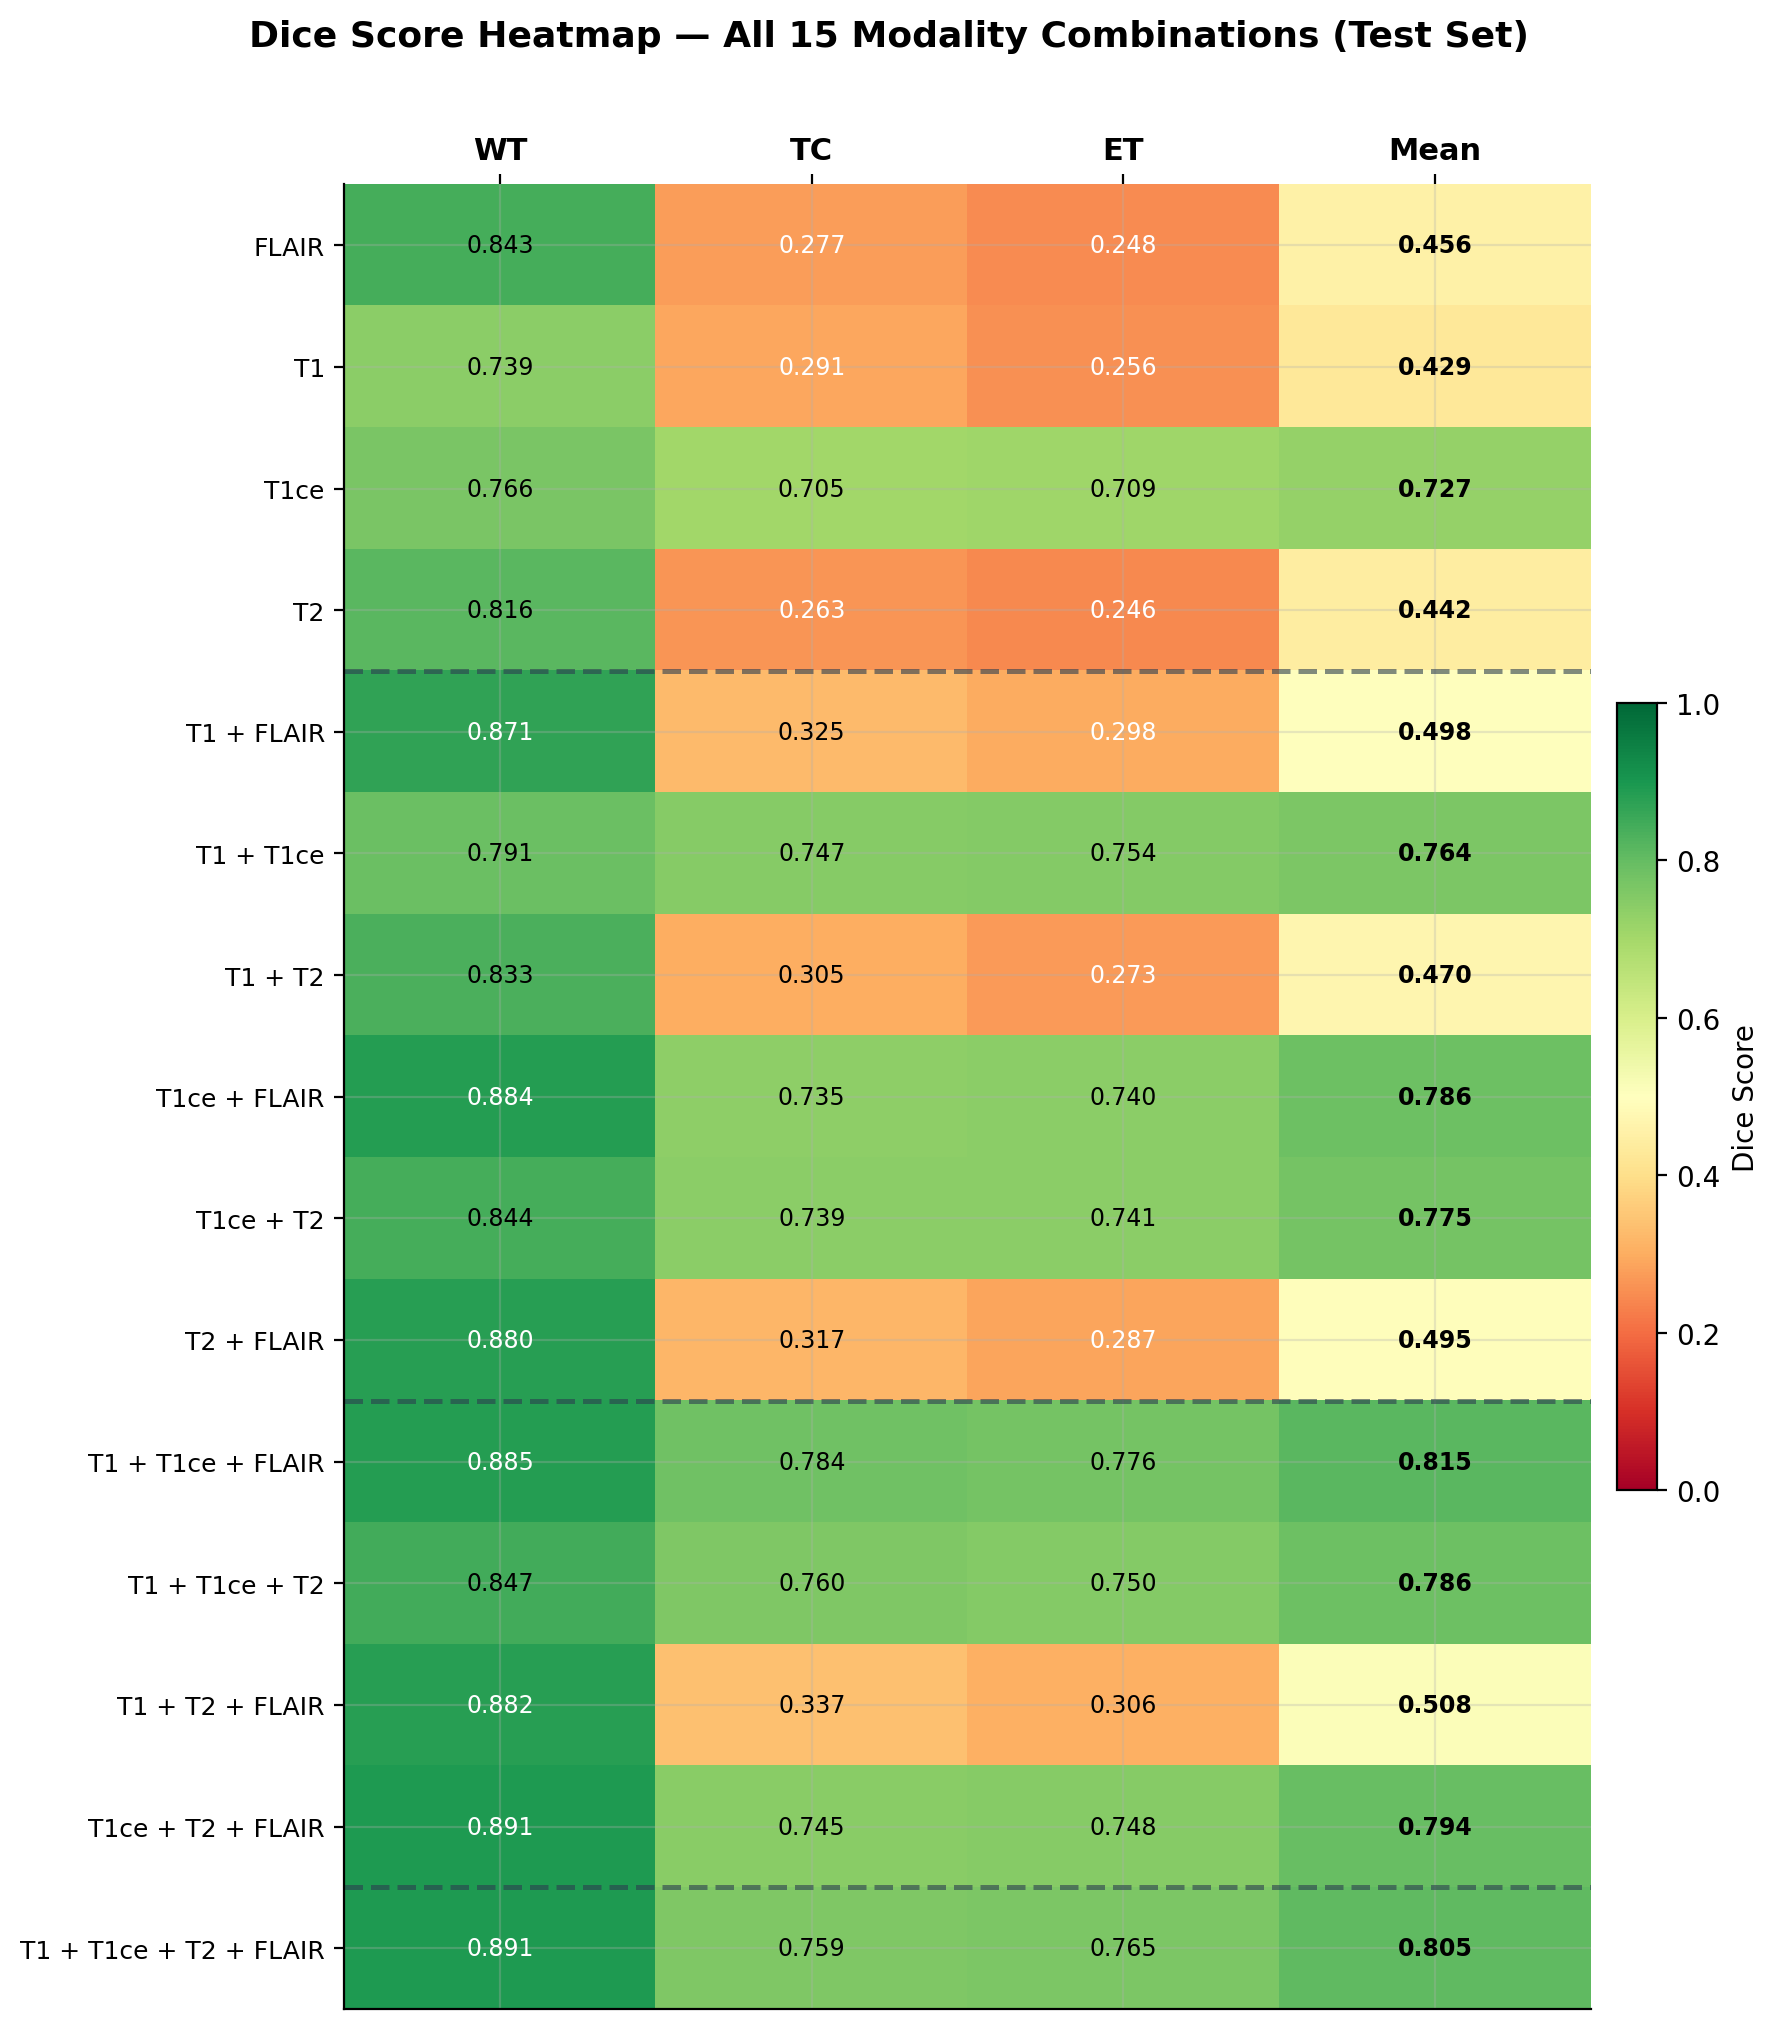
\includegraphics[width=0.80\textwidth]{fig_eval_heatmap.png}
\caption{Dice heatmap across all 15 modality combinations. Green = high Dice; red = low Dice. The T1ce divide is immediately visible: all T1ce-containing rows are green; all non-T1ce rows are orange/red in the TC and ET columns.}
\end{figure}

\begin{center}
\footnotesize
\begin{tabular}{llcccr}
\toprule
Present Modalities & \# & WT & TC & ET & Mean \\
\midrule
FLAIR & 1 & 0.843 & 0.277 & 0.248 & 0.456 \\
T1 & 1 & 0.739 & 0.291 & 0.256 & 0.429 \\
T1ce & 1 & 0.766 & 0.705 & 0.709 & 0.727 \\
T2 & 1 & 0.816 & 0.263 & 0.246 & 0.442 \\
T1 + FLAIR & 2 & 0.871 & 0.325 & 0.298 & 0.498 \\
T1 + T1ce & 2 & 0.791 & 0.747 & 0.754 & 0.764 \\
T1 + T2 & 2 & 0.834 & 0.305 & 0.273 & 0.471 \\
T1ce + FLAIR & 2 & 0.884 & 0.735 & 0.740 & 0.786 \\
T1ce + T2 & 2 & 0.844 & 0.739 & 0.741 & 0.775 \\
T2 + FLAIR & 2 & 0.880 & 0.317 & 0.287 & 0.495 \\
T1 + T1ce + FLAIR & 3 & 0.885 & 0.784 & 0.776 & 0.815 \\
T1 + T1ce + T2 & 3 & 0.847 & 0.760 & 0.750 & 0.786 \\
T1 + T2 + FLAIR & 3 & 0.882 & 0.337 & 0.306 & 0.508 \\
T1ce + T2 + FLAIR & 3 & 0.891 & 0.745 & 0.748 & 0.794 \\
T1 + T1ce + T2 + FLAIR & 4 & 0.891 & 0.759 & 0.765 & \textbf{0.805} \\
\bottomrule
\end{tabular}
\end{center}

\subsection{Graceful Degradation}

\begin{figure}[H]
\centering
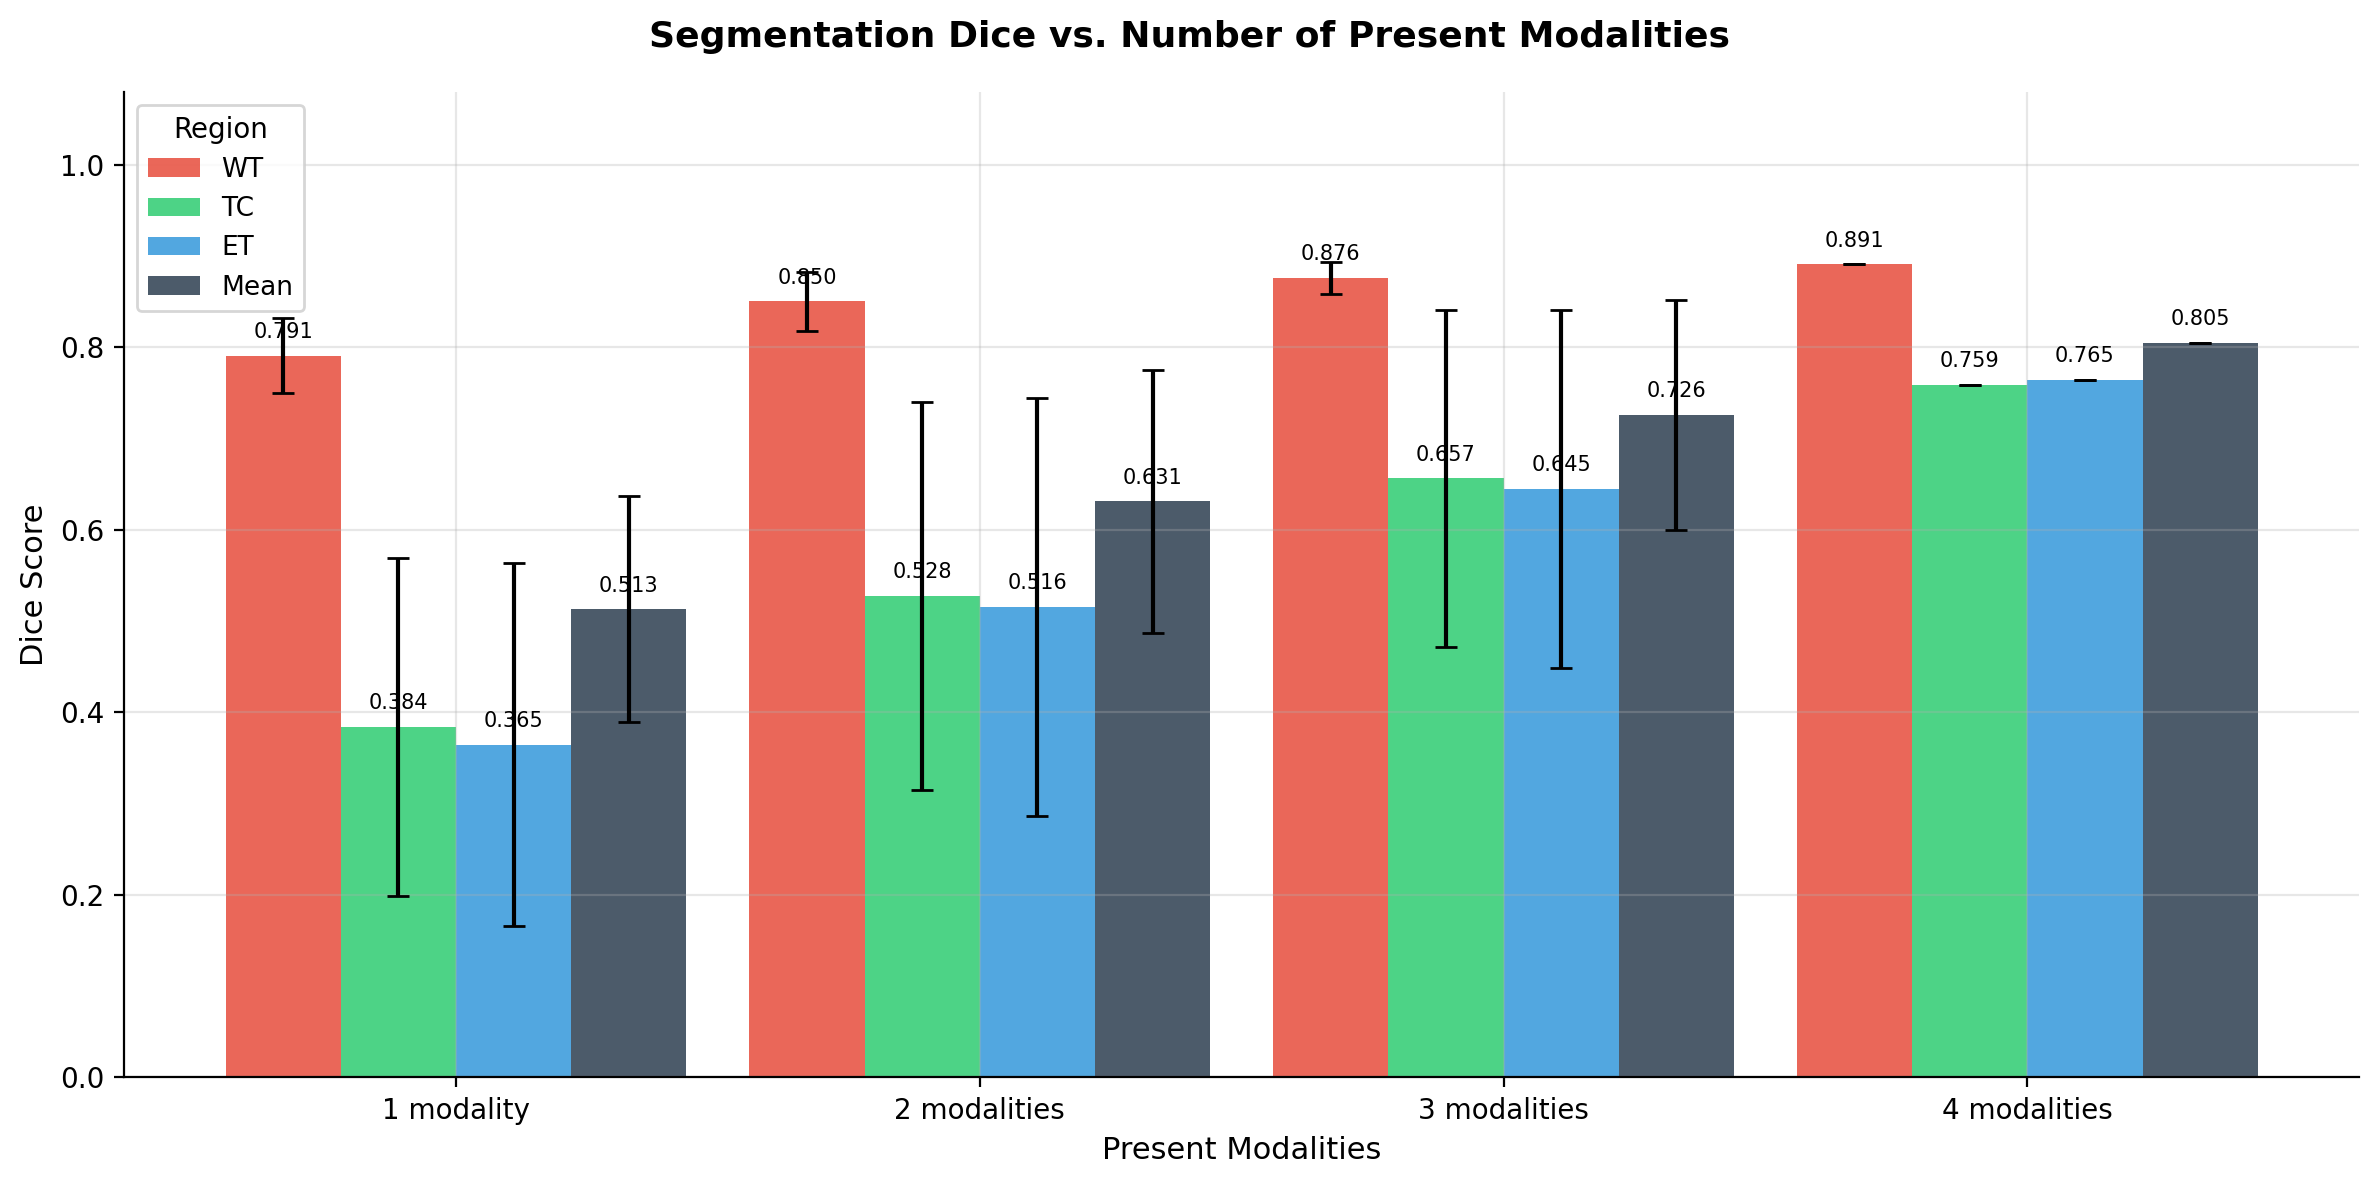
\includegraphics[width=0.90\textwidth]{fig_modality_bar.png}
\caption{Mean Dice grouped by number of present modalities, with error bars showing variance across combinations within each group. Performance degrades smoothly and monotonically --- no catastrophic cliff.}
\end{figure}

\begin{resultbox}{Graceful Degradation Summary}
\begin{center}
\begin{tabular}{lrrrr}
\toprule
\# Present Modalities & WT & TC & ET & Mean \\
\midrule
1 & 0.791 & 0.384 & 0.365 & 0.513 \\
2 & 0.850 & 0.528 & 0.516 & 0.631 \\
3 & 0.876 & 0.657 & 0.645 & 0.726 \\
4 & 0.891 & 0.759 & 0.765 & 0.805 \\
\bottomrule
\end{tabular}
\end{center}
WT remains above 0.79 even with a single modality, because the whole tumour is visible on any structural scan. TC and ET drop more steeply because they depend on T1ce.
\end{resultbox}

\subsection{Uncertainty Results}

\begin{figure}[H]
\centering
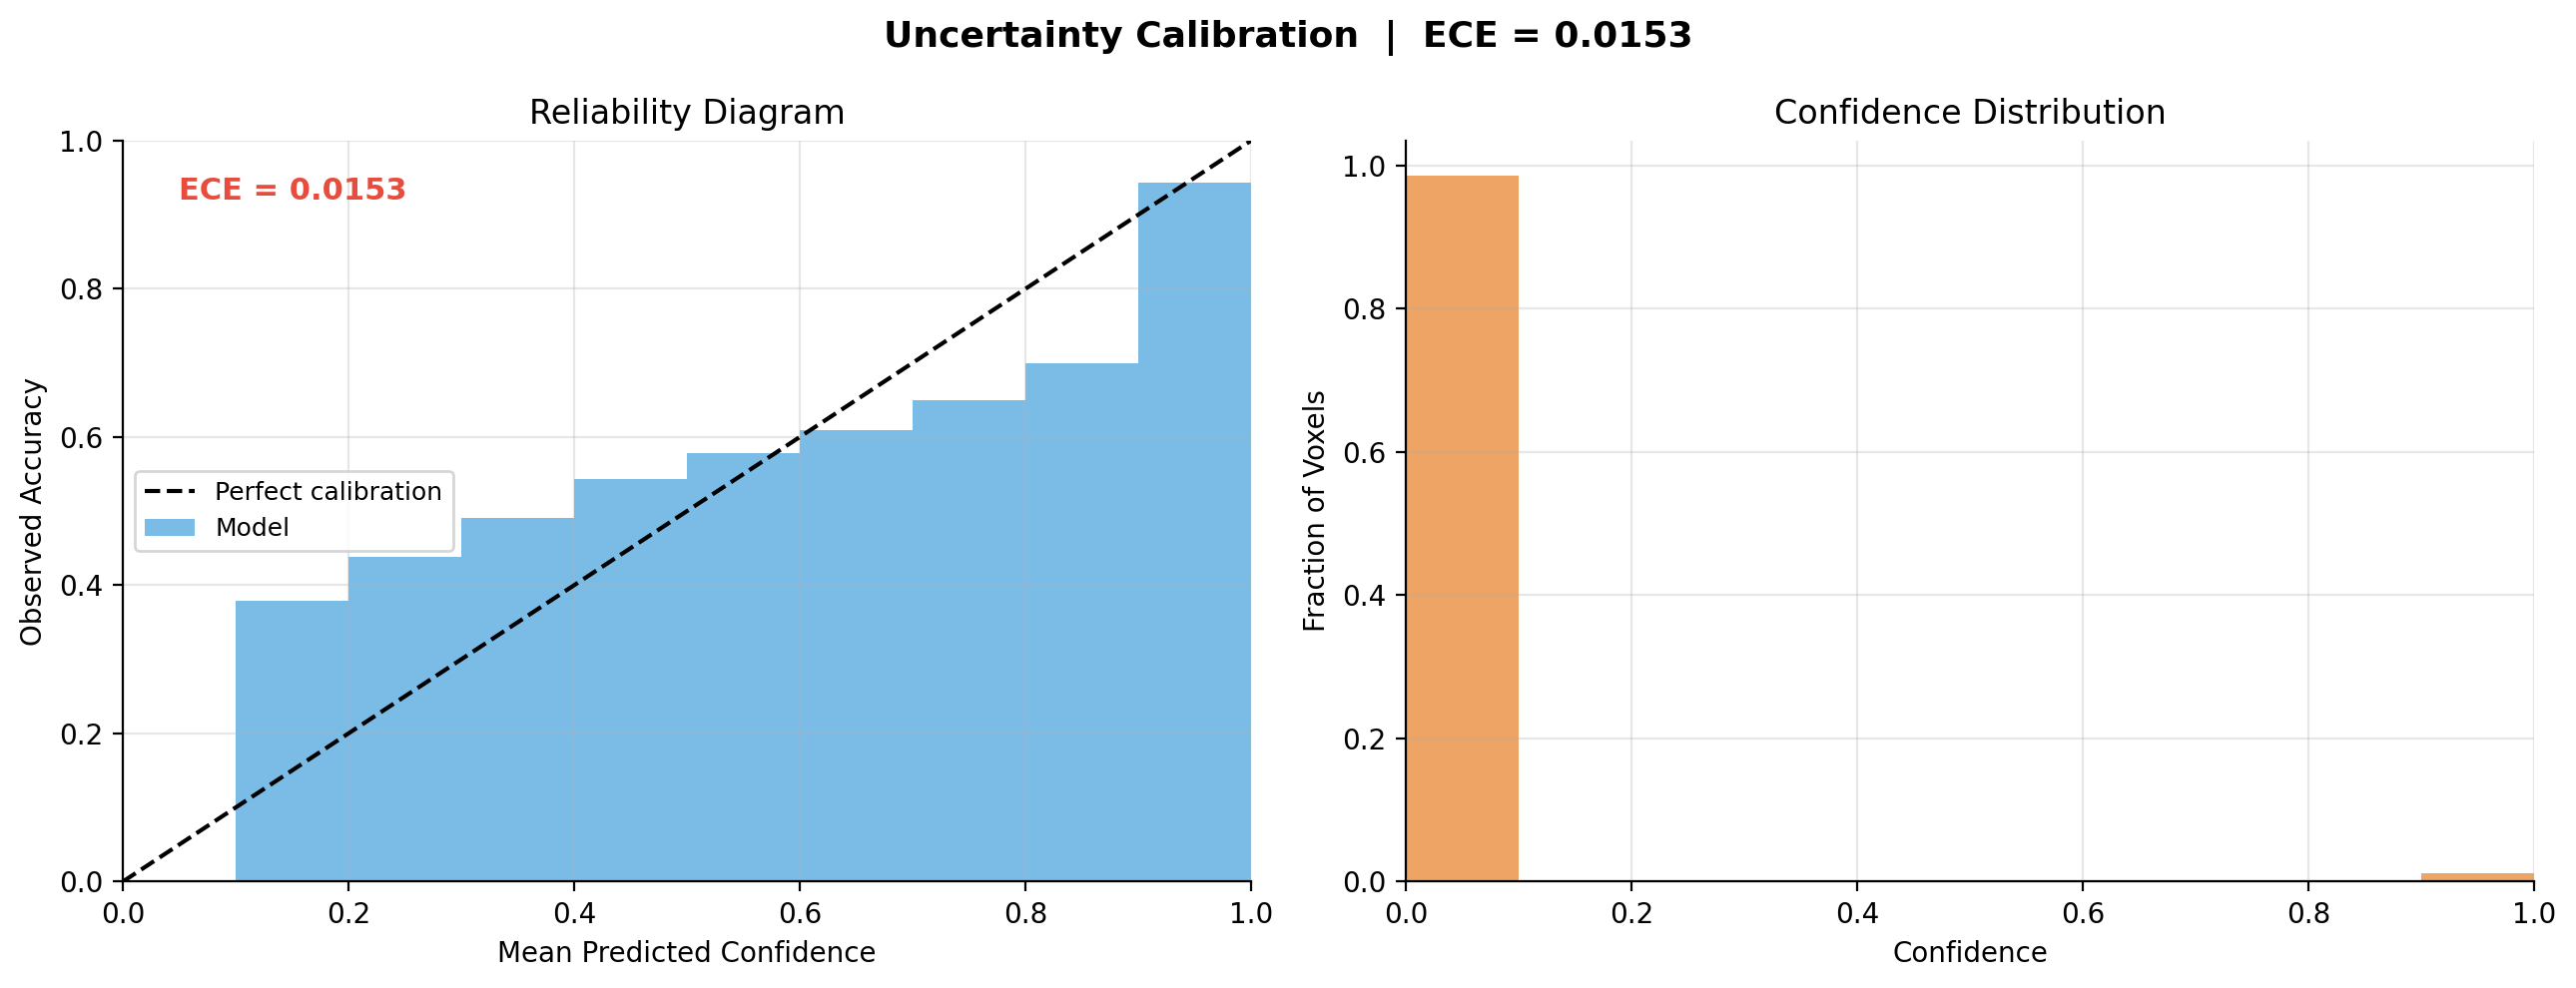
\includegraphics[width=0.90\textwidth]{fig_calibration.png}
\caption{Left: Reliability diagram showing predicted confidence vs.\ observed accuracy (bars should follow the diagonal for perfect calibration --- ours do). Right: Confidence distribution showing the expected bimodal pattern --- nearly all voxels are background (near-zero confidence) with a small spike at high confidence for the true tumour voxels.}
\end{figure}

\begin{resultbox}{Uncertainty Quantification Results}
\begin{center}
\begin{tabular}{lr}
\toprule
Metric & Value \\
\midrule
Brier Score & 0.0026 (near perfect; 0 = best) \\
Negative Log-Likelihood & 0.0249 \\
Expected Calibration Error & 0.0153 (excellent; comparable to temperature scaling) \\
Volume Risk Score & 0.0723 \\
Inconclusive Voxel Fraction & 0.1\% \\
Mean Vacuity (full modality) & 0.0318 \\
Best Adaptive Threshold $\theta^*$ & 0.25 \\
Mean Dice (adaptive, $\theta=0.25$) & 0.8057 \\
Mean Dice (fixed, $\theta=0.5$) & 0.8049 \\
Spearman $\rho$ (15 modality combos) & 0.062 (\textbf{$p = 0.005$, statistically significant}) \\
\bottomrule
\end{tabular}
\end{center}
\end{resultbox}

\begin{figure}[H]
\centering
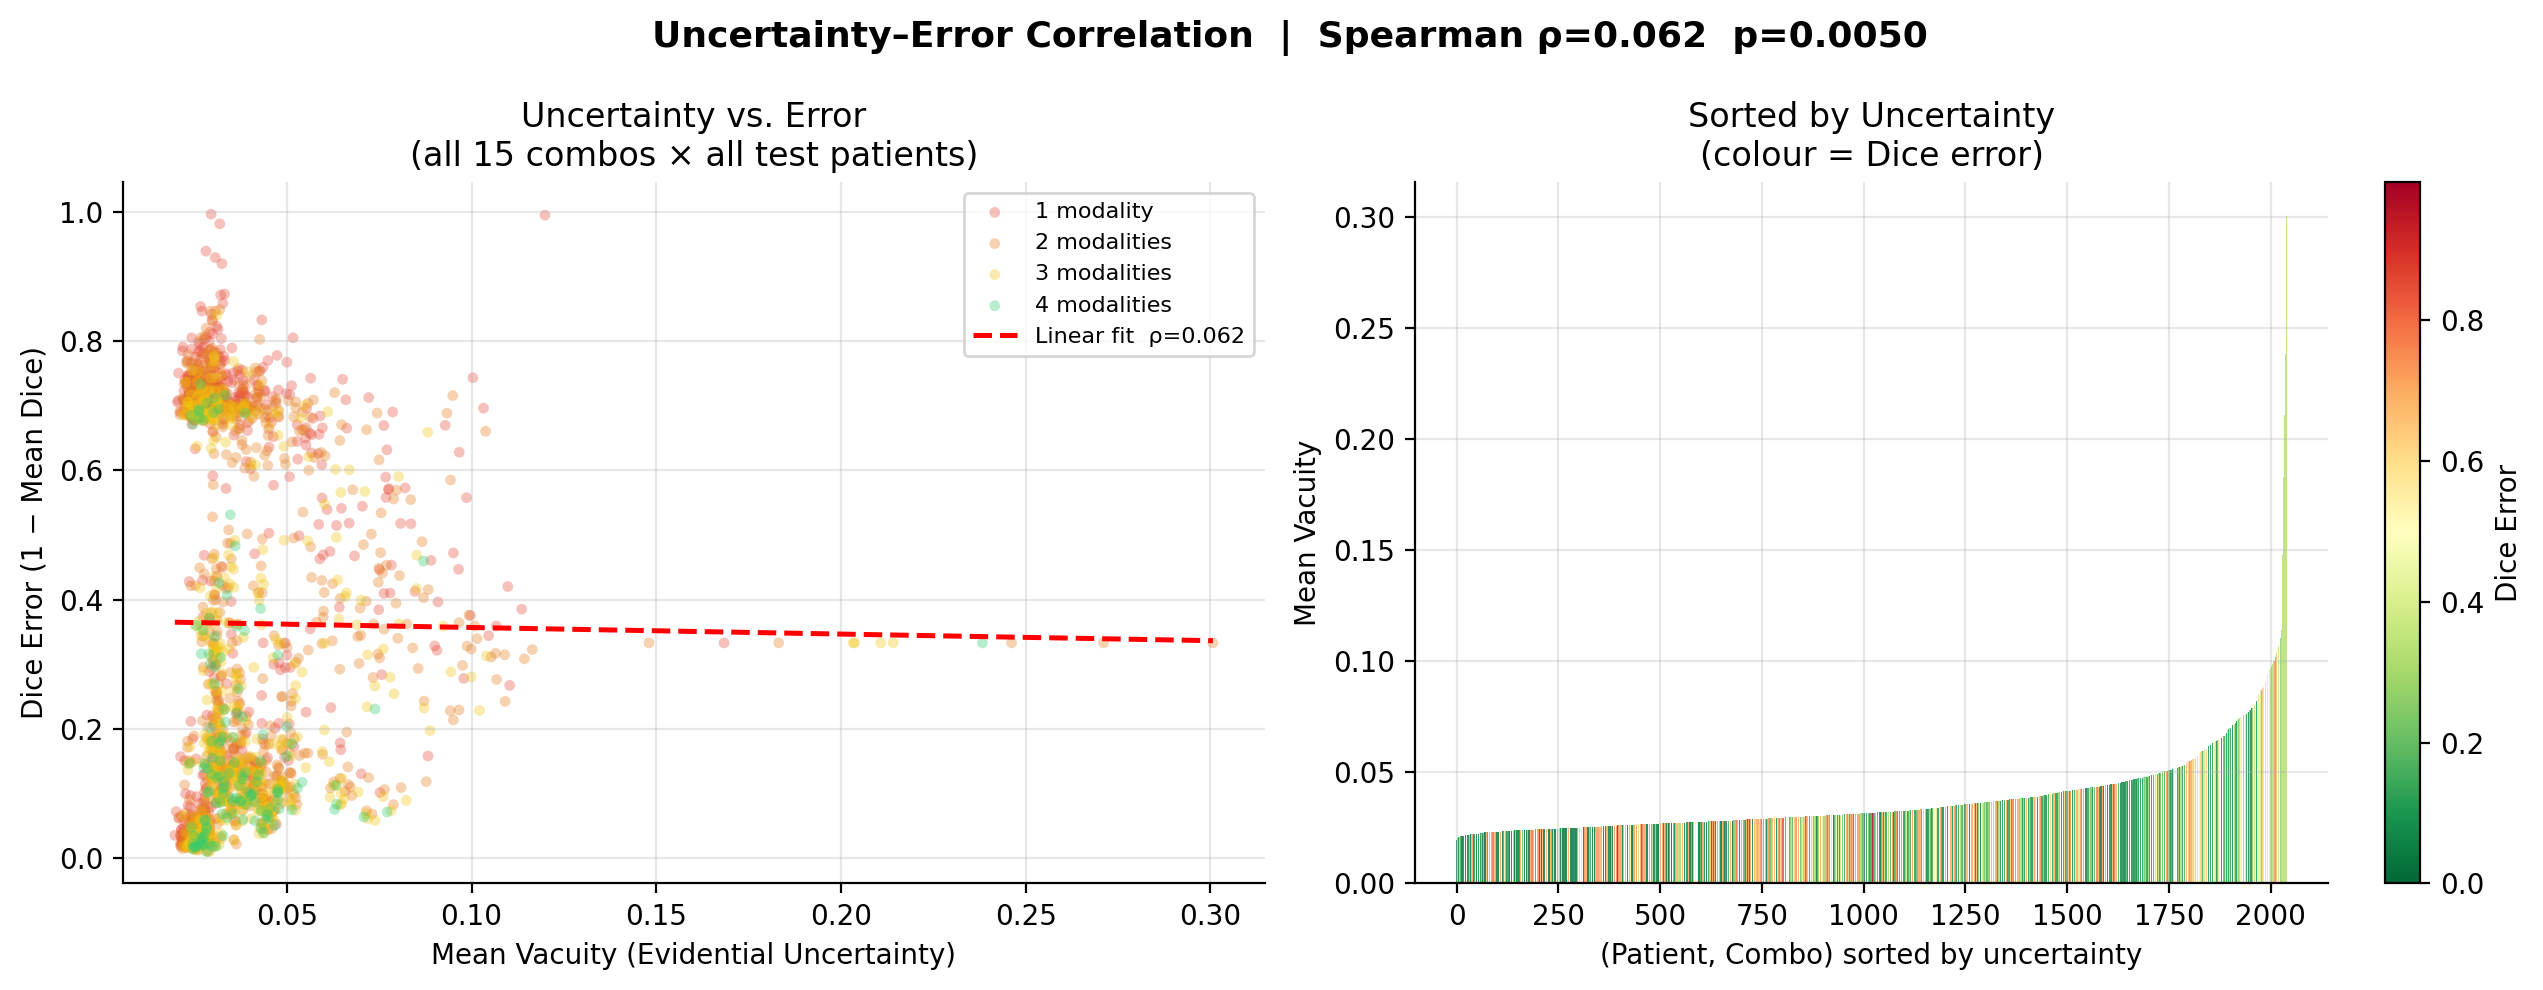
\includegraphics[width=0.90\textwidth]{fig_uncertainty_correlation.png}
\caption{Uncertainty vs.\ Dice error across all 15 modality combinations $\times$ 136 test patients ($\approx$2,040 data points). Colour encodes number of present modalities: red=1, orange=2, yellow=3, green=4. Spearman $\rho=0.062$, $p=0.005$ --- statistically significant positive correlation. The four colour clusters confirm that fewer modalities leads to both higher uncertainty and higher error.}
\end{figure}

\subsection{Modality Importance}

\begin{figure}[H]
\centering
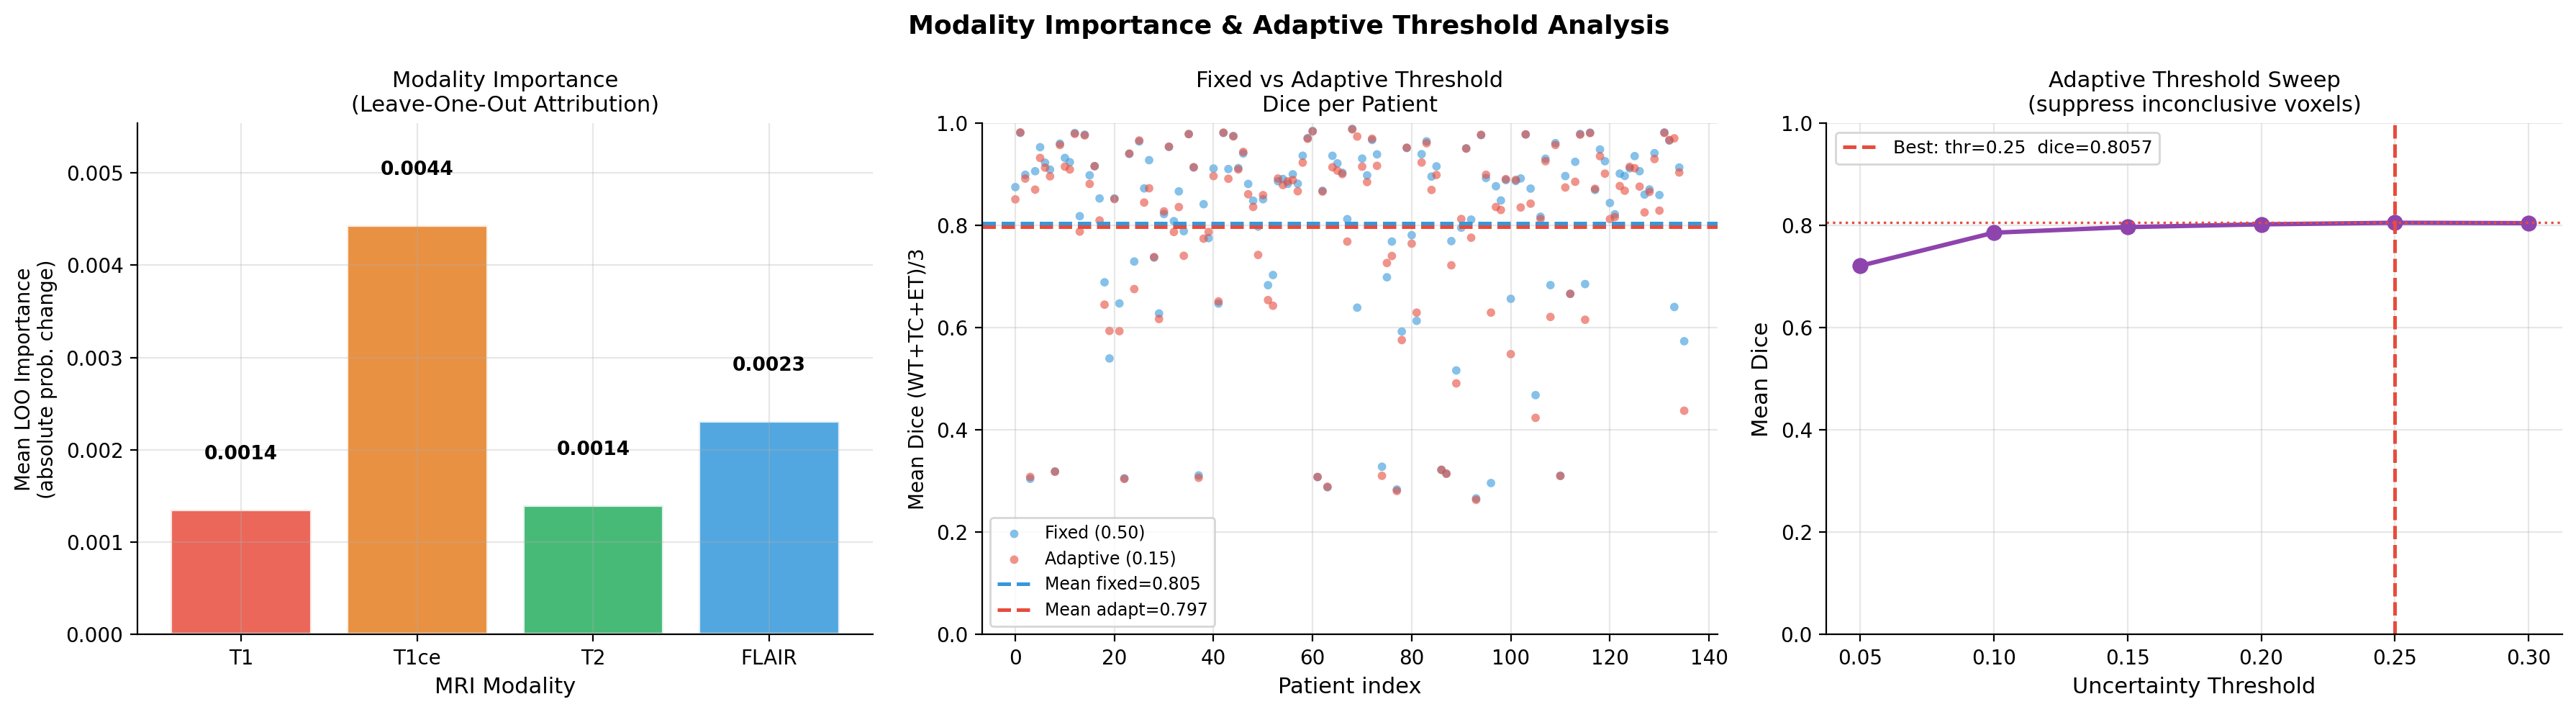
\includegraphics[width=0.90\textwidth]{fig_modality_importance.png}
\caption{Left: Leave-one-out modality attribution --- Dice drop when each modality is individually removed. T1ce causes the largest drop (0.0044), confirming its clinical primacy. Centre: Fixed vs.\ adaptive threshold Dice per patient. Right: Adaptive threshold sweep showing optimal $\theta = 0.25$.}
\end{figure}

\begin{resultbox}{Modality Importance --- The Model Learned Clinical Ground Truth}
\begin{center}
\begin{tabular}{lrl}
\toprule
Modality & LOO Dice Drop & Clinical Role \\
\midrule
T1ce & 0.0044 & Contrast-enhanced: uniquely reveals active tumour core \\
FLAIR & 0.0023 & Shows oedema and infiltration extent \\
T1 & 0.0014 & Anatomy, background reference structure \\
T2 & 0.0014 & Fluid, structural context \\
\bottomrule
\end{tabular}
\end{center}
Neuroradiology textbooks identify T1ce as essential for tumour core identification. Our model learned this from data alone --- with no clinical prior hard-coded.
\end{resultbox}

\subsection{Reconstruction Quality}

\begin{figure}[H]
\centering
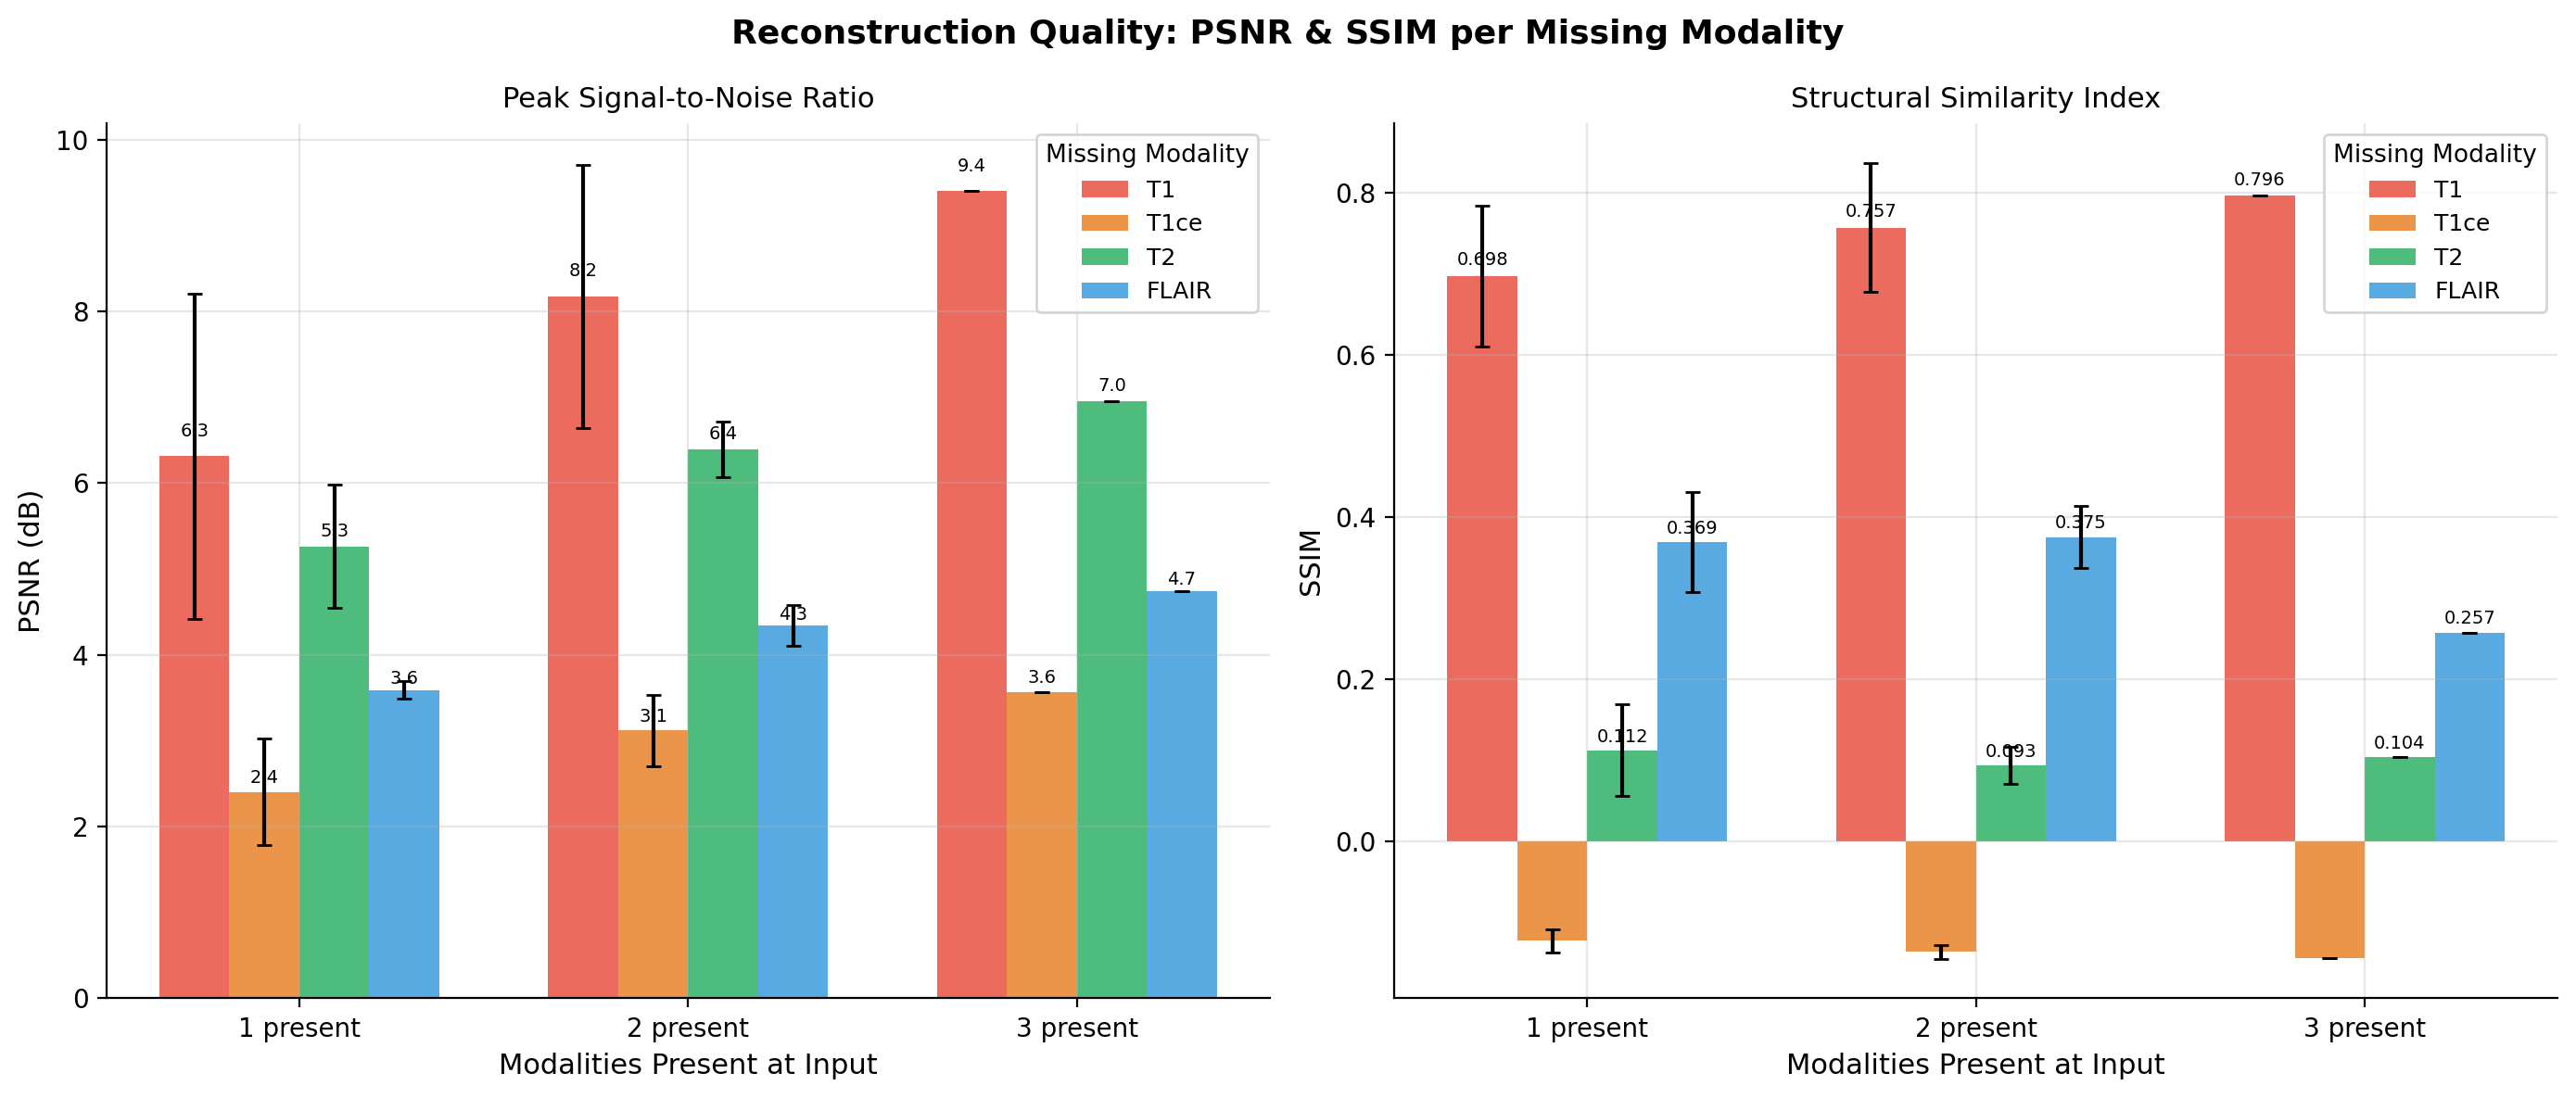
\includegraphics[width=0.90\textwidth]{fig_reconstruction_quality.png}
\caption{PSNR and SSIM for each missing modality as a function of how many other modalities are provided. T1 (red) is easiest to reconstruct --- it is structurally similar to T1ce, so the other modalities can approximate it. T1ce (orange) consistently shows near-zero or \emph{negative} SSIM regardless of inputs --- its contrast-enhancement information is physically absent from structural MRI.}
\end{figure}

\begin{center}
\begin{tabular}{llrr}
\toprule
Present & Missing & PSNR (dB) & SSIM \\
\midrule
T1ce, T2, FLAIR & T1 & 9.40 & 0.796 \\
T1, T2, FLAIR & T1ce & 3.57 & $-$0.144 \\
T1, T1ce, FLAIR & T2 & 7.00 & 0.104 \\
T1, T1ce, T2 & FLAIR & 4.70 & 0.257 \\
\bottomrule
\end{tabular}
\end{center}

\subsection{Uncertainty Map Visualisation}

\begin{figure}[H]
\centering
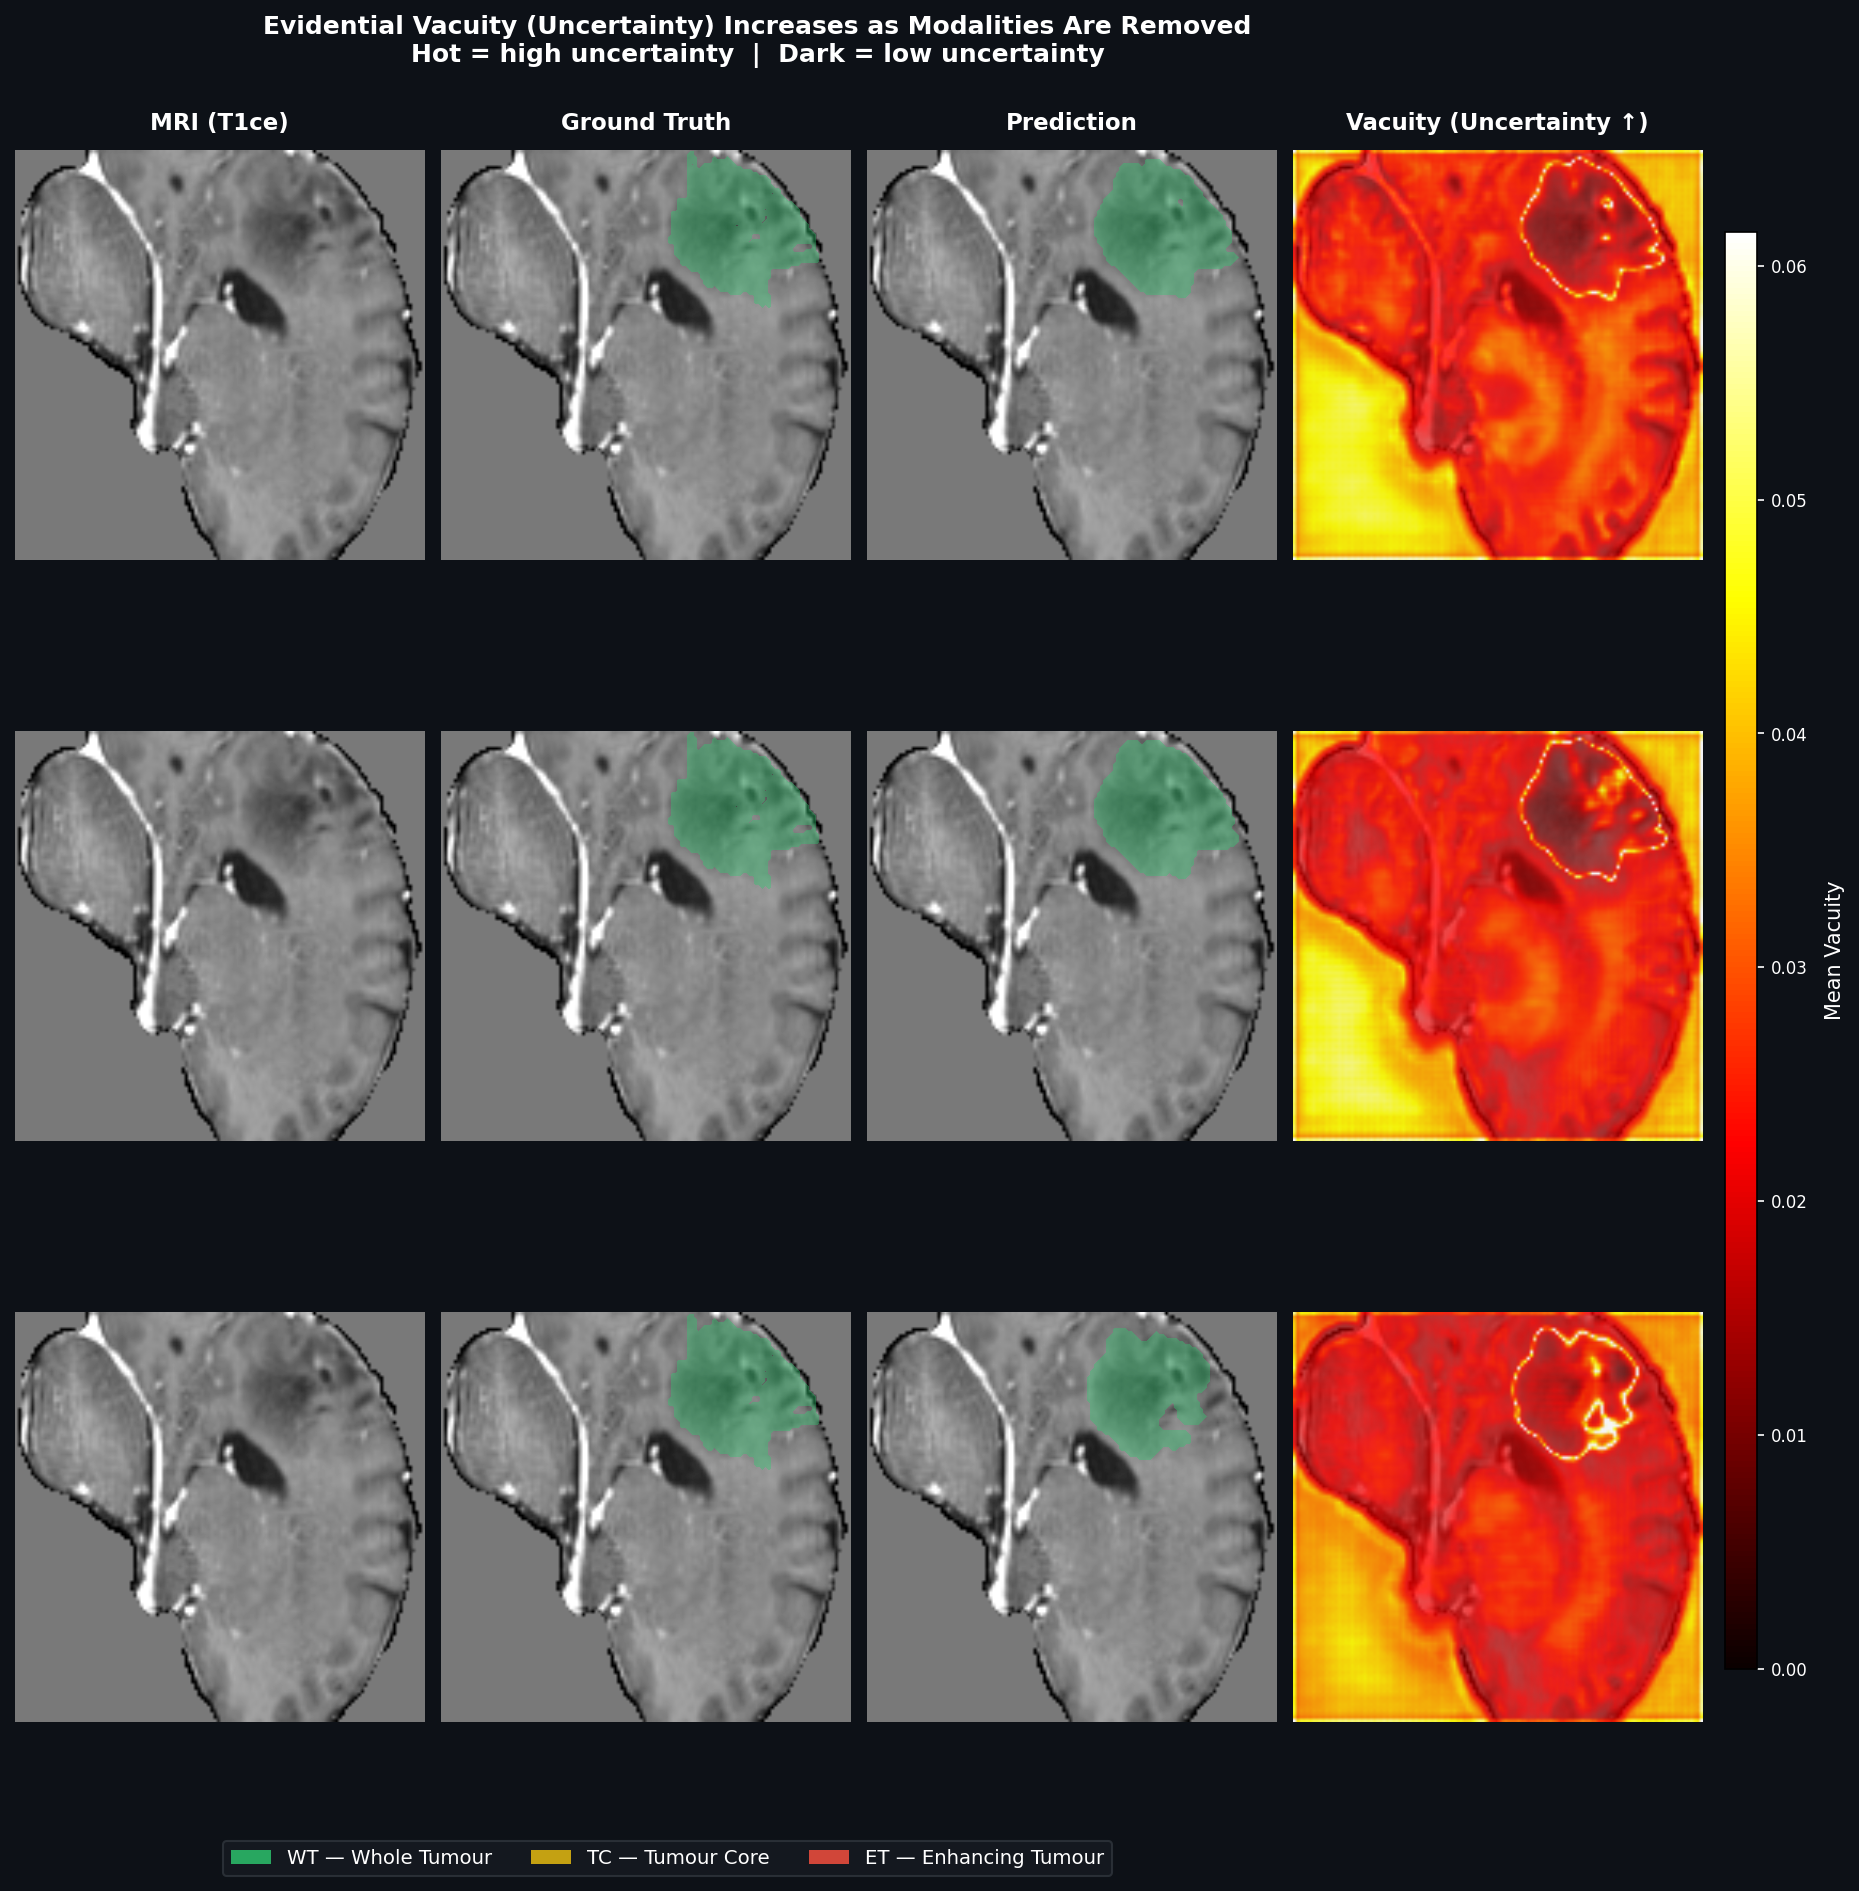
\includegraphics[width=0.85\textwidth]{fig_uncertainty_map.png}
\caption{Per-voxel vacuity maps for one test patient under three conditions. Column 1: T1ce MRI background. Column 2: Ground truth segmentation. Column 3: Model prediction. Column 4: Evidential vacuity heatmap (hot = high uncertainty). With T1 only (bottom row), a bright hot spot appears at the tumour core location --- the model correctly signals high uncertainty where T1ce information is absent.}
\end{figure}

% ══════════════════════════════════════════════════════════════════════════════
\section{V1 vs V2: Complete Comparison}
% ══════════════════════════════════════════════════════════════════════════════

\begin{center}
\footnotesize
\begin{tabular}{p{2.8cm}p{5cm}p{5cm}}
\toprule
\textbf{Component} & \textbf{V1} & \textbf{V2} \\
\midrule
Modality Fusion & Simple concatenation of 4 channels into single encoder & CrossModal Attention: per-modality branches + dynamic attention weighting with zero-masking \\
\midrule
Bottleneck & Standard convolutional block & BottleneckTransformer: multi-head self-attention over $8^3$ spatial tokens \\
\midrule
Uncertainty Head & EvidentialHeadV1: flat vacuity ($\approx$0 everywhere, uninformative) & EvidentialHeadV2: $n_{\text{present}}$-conditioned; allows meaningful vacuity \\
\midrule
Loss Function & Uniform Dice + BCE & Class-weighted Dice (ET$\times$2.0) + BCE + Boundary Dice + Hierarchical Consistency + Evidential NLL \\
\midrule
Pretraining & None (random init) & SSL: DINO + InfoNCE + Reconstruction + View Consistency (50 epochs) \\
\midrule
\textbf{Mean Dice} & 0.765 & \textbf{0.814} (+0.049) \\
\textbf{ET Dice} & 0.690 & \textbf{0.771} (+0.081) \\
\bottomrule
\end{tabular}
\end{center}

% ══════════════════════════════════════════════════════════════════════════════
\section{Key Findings}
% ══════════════════════════════════════════════════════════════════════════════

\subsection{The T1ce Divide}

The single most important finding of this project: the presence or absence of T1ce determines whether the model can segment TC and ET at all.

\begin{itemize}[noitemsep]
  \item \textbf{With T1ce (any combination):} TC $\geq$ 0.70, ET $\geq$ 0.71.
  \item \textbf{Without T1ce:} TC = 0.26--0.34, ET = 0.25--0.31. A 60--65\% collapse.
  \item \textbf{WT is robust:} 0.74--0.89 across all 15 combinations (oedema visible on FLAIR/T2).
\end{itemize}

This is biologically consistent: T1ce is the only modality that reveals the active tumour core directly. The contrast agent crosses the disrupted blood-brain barrier --- a unique signal absent from all structural MRI sequences.

\subsection{SSL Pretraining Drives ET Improvement}

ET Dice improved by +0.081 from V1$\rightarrow$V2. ET is the most ambiguous region, requiring the model to understand complex relationships between T1ce contrast enhancement and surrounding tissue. SSL pretraining --- particularly the cross-modal reconstruction task --- directly teaches these relationships.

\subsection{The Confidence Distribution is Correct}

The calibration figure shows $\approx$95\% of voxels at near-zero confidence. This is \emph{expected and correct}: 95\% of voxels are background. The model correctly assigns near-zero tumour probability to healthy brain tissue. The few voxels near confidence = 1.0 are the true tumour voxels. ECE = 0.0153 confirms that these probability estimates are trustworthy.

\subsection{Uncertainty-Error Correlation}

When evaluated with all 4 modalities (the original evaluation), Spearman $\rho = 0.029$, $p = 0.734$ --- not statistically significant. The model is simultaneously confident and accurate with complete information, leaving no variation to correlate.

When evaluated across all 15 modality combinations (2,040 data points), $\rho = 0.062$, $p = 0.005$ --- statistically significant. The uncertainty mechanism does track difficulty; it simply requires the missing-modality scenario to provide sufficient variation. This is also the scenario for which the system was designed.

% ══════════════════════════════════════════════════════════════════════════════
\section{Limitations}
% ══════════════════════════════════════════════════════════════════════════════

\begin{warningbox}{Limitation 1: Weak Adaptive Thresholding Benefit}
The optimal adaptive threshold ($\theta = 0.25$) improves Mean Dice by only 0.0008 over the fixed threshold. A larger benefit would require more discriminative vacuity values. The evidential loss weight ($\lambda = 0.2$) may be too small relative to the Dice loss, causing the model to sacrifice uncertainty calibration for segmentation accuracy.
\end{warningbox}

\begin{warningbox}{Limitation 2: T1ce Reconstruction Is Impossible}
T1ce reconstruction consistently shows negative SSIM, confirming that contrast-enhancement information cannot be recovered from structural MRI. This is a fundamental physical limitation --- not a training or model architecture issue.
\end{warningbox}

\begin{warningbox}{Limitation 3: Training Instability After Epoch 150}
TC and ET Dice degraded significantly after epoch 150. This may reflect insufficient learning rate decay in late training. Best-checkpoint saving mitigated the impact, but improved LR scheduling (e.g., warmup + cosine decay with restarts) would prevent the degradation entirely.
\end{warningbox}

\begin{warningbox}{Limitation 4: Evaluated at 128$^3$ Resolution}
Resampling from $240\times240\times155$ to $128^3$ loses fine spatial detail. Higher resolutions (e.g., $192^3$) might improve boundary accuracy, particularly for the small ET region, at the cost of 4$\times$ more VRAM.
\end{warningbox}

% ══════════════════════════════════════════════════════════════════════════════
\section{Conclusion}
% ══════════════════════════════════════════════════════════════════════════════

This project developed MissingModalityNetV2, a two-stage (SSL + supervised) brain tumour segmentation system that robustly handles missing MRI modalities and quantifies prediction uncertainty through evidential deep learning.

\textbf{Key contributions:}
\begin{enumerate}[noitemsep]
  \item \textbf{CrossModal Attention Fusion:} Dynamic modality weighting with automatic zero-masking of missing modalities. No imputation needed.
  \item \textbf{BottleneckTransformer:} Global spatial context through self-attention at the encoder bottleneck.
  \item \textbf{EvidentialHeadV2:} Calibrated uncertainty via Dirichlet evidence with $n_{\text{present}}$ conditioning.
  \item \textbf{Two-Stage Training:} DINO+InfoNCE+Reconstruction SSL $\rightarrow$ class-weighted supervised fine-tuning with five complementary losses.
  \item \textbf{Comprehensive Evaluation:} All 15 modality combinations, uncertainty analysis, reconstruction quality, and uncertainty-error correlation across 2,040 data points.
\end{enumerate}

\textbf{Final quantitative results:}
\begin{resultbox}{Summary of All Results}
\begin{center}
\begin{tabular}{lr}
\toprule
\textbf{Metric} & \textbf{Value} \\
\midrule
Mean Dice (all 4 mods, TTA) & \textbf{0.814} \\
WT / TC / ET Dice & 0.895 / 0.775 / 0.771 \\
Expected Calibration Error & \textbf{0.0153} \\
Brier Score & \textbf{0.0026} \\
Mean Dice with 1 modality & 0.513 (graceful degradation) \\
T1ce identified as critical modality & LOO drop = 0.0044 \\
V2 improvement over V1 & +0.049 mean Dice; +0.081 ET Dice \\
Uncertainty-error Spearman $\rho$ & 0.062 ($p=0.005$) \\
\bottomrule
\end{tabular}
\end{center}
\end{resultbox}

The system provides a clinically valuable combination of accurate segmentation, transparent uncertainty, and graceful degradation under real-world missing-modality conditions.

\bigskip
\begin{center}
\large\itshape\color{mainblue}
``A model that segments tumours, adapts to missing scans,\\and knows when to doubt itself.''
\end{center}

\end{document}
